\documentclass[a4paper,cleardoubleempty,BCOR1cm]{scrbook}
% use to waste space:
% \documentclass[12pt,a4paper]{article}

% if you have this style and like it.
%\documentclass{acmsiggraph}
%\documentclass[review]{acmsiggraph}      % review
%\documentclass[widereview]{acmsiggraph}  % wide-spaced review
%\documentclass[preprint]{acmsiggraph}    % preprint

% define a \comment{this is a comment which can have linebreaks in it}
\newcommand{\comment}[1]{}
% \newcommand{\todo}[1]{\marginpar{\bf{#1}}}
\newcommand{\todo}[1]{{\color{red}\bf{TODO: #1}}}

\usepackage{mathptmx}
\usepackage[pdftex]{graphicx}
\usepackage[pdftex]{color}
\definecolor{rot}{RGB}{165,30,55} %rote Farbe
\graphicspath{{./images/}}
\usepackage{parskip}
\usepackage{amsmath}
% \usepackage{dsfont}
\usepackage{pxfonts}

\usepackage[T1]{fontenc}
\usepackage{textcomp}

% comment these two lines out if you don't want minion/myriad fonts.
% \usepackage[minionint,mathlf]{MinionPro}
% \renewcommand{\sfdefault}{Myriad-LF}
%\usepackage{Myriad}

% no page number on float pages, fixes problems with overlarge diagrams.
\usepackage{fancyhdr}
\pagestyle{fancy}
%\lhead{}
%\chead{}
%\rhead{}
%\lfoot{}
\fancyhf{}
\fancyhead[EL]{\nouppercase{\leftmark}}
\fancyhead[OR]{\nouppercase{\rightmark}}
\cfoot{}
%\fancyfoot[EL]{\iffloatpage{}{\thepage}}
%\fancyfoot[OR]{\iffloatpage{}{\thepage}}
\fancyfoot[EL]{\thepage}
\fancyfoot[OR]{\thepage}
\renewcommand{\headrulewidth}{0pt}
\renewcommand{\footrulewidth}{0pt}

%\usepackage{natbib}		% textual referencing
%\usepackage[numbers,super]{natbib}	% nice superscripts
%\bibliographystyle{chicago}	% shitty
\bibliographystyle{alpha}	% abbr names and year in \cite
%\bibliographystyle{agsm}	% australian, need natbib
%\bibliographystyle{kluwer}	% need natbib
%\bibliographystyle{apalike}	% lengthly
%\bibliographystyle{abbrv}	% minimal?

% use for german line breaking:
%\usepackage[ngerman]{babel}
\usepackage[T1]{fontenc}
\usepackage[utf8x]{inputenc}

% avoid us-style text color destruction:
\frenchspacing
\usepackage{microtype}

% have a nice framebox with border directly around the image:
\fboxsep 0pt
\newcommand{\fimg}[2]{\fbox{\includegraphics[width=#1]{#2}}}

\usepackage{theorem}
\theorembodyfont{\upshape}
\newtheorem{definition}{Definition}

\usepackage{listings}
\lstset{numbers=left, numberstyle=\tiny, basicstyle=\tiny, language=C++}
\usepackage[boxruled]{algorithm2e}
%\usepackage{hyperref}
\usepackage{url}
\usepackage{subfig}

\def\code#1{{\tt{#1}}}



\title{Bachelorarbeit}
\author{Peter Trost \thanks{e-mail: peter.trost@student.uni-tuebingen.de}}
\date{\today}
\begin{document}

\begin{tabular}{lr}
% 
\includegraphics[width=0.5\linewidth]{logo_sw} % logo bw
 
\includegraphics[width=0.5\linewidth]{UT_WBMW_Rot_4C} % logo red
 & \hspace{0.2\linewidth}
 \parbox{0.5\linewidth}{
   \large\bf\textsf{\color{rot}{Mathematisch-\\Naturwissenschaftliche\\Fakultät\\\\}}
  \hspace{-.144cm}\normalsize\textsf{\color{rot}{Lernbasierte Computer Vision}}
   \vspace{0.6cm}
 }
\end{tabular}

\vspace*{10ex}
Bachelorarbeit

{\huge\bf\textsf{A Comparison of Synthetic-to-Real Domain Adaptation Techniques}}

\vspace*{30ex}

Eberhard Karls Universität Tübingen\\
Mathematisch-Naturwissenschaftliche Fakultät\\
Wilhelm-Schickard-Institut für Informatik\\
Lernbasierte Computer Vision\\
Peter Trost,~ \verb+peter.trost@student.uni-tuebingen.de+,~ 2019

\vspace*{5ex}

\begin{tabular}{@{}l@{\hspace{2em}}l}
  Bearbeitungszeitraum:& 24.05.2019-23.09.2019 \vspace*{5ex} \\
  Betreuer/Gutachter:& Prof. Dr. Andreas Geiger, Universität Tübingen\\
  					 &Despoina Paschalidou, ETH Zürich\\
  					 &Dr. Yiyi Liao, Max-Planck-Institut für Intelligente Systeme Tübingen
\end{tabular}

\thispagestyle{empty}
\newpage

\chapter*{Selbstst\"andigkeitserkl\"arung}
Hiermit versichere ich, dass ich die vorliegende Bachelorarbeit selbst\"andig und
nur mit den angegebenen Hilfsmitteln angefertigt habe und dass alle Stellen,
die dem Wortlaut oder dem Sinne nach anderen Werken entnommen sind,
durch Angaben von Quellen als Entlehnung kenntlich gemacht worden sind.
Diese Bachelorarbeit wurde in gleicher oder \"ahnlicher Form in keinem anderen
Studiengang als Pr\"ufungsleistung vorgelegt.

\vspace*{8ex}
\hrule
\vspace*{2ex}
Peter Trost (Matrikelnummer 4039682), \today



\chapter*{Abstract}
With autonomous driving being very popular and gaining a lot of publicity these days there is lots of money and research going into the topic of Artificial Neural Networks that decide how to drive these autonomous vehicles. Currently Deep Neural Networks are the go to architecture used for this task. These Networks need large amounts of data to learn how to properly classify objects in the driving environment so the system can make the right decisions. Currently the best results in training are achieved through supervised training, i.e. having the expected output (ground truth) for each given input. Creating datasets for autonomous driving applications that contain real world images and accurate ground truth is time intensive and therefore very costly. In contrast there are many approaches that can cheaply generate loads of synthetic images from virtual worlds with accurate pixel-level labeling. Models that are trained on these synthetic datasets however perform worse in the real world due to the domain shift (changes in texture, lighting,...) between the synthetic and real domain. The research area of Domain Adaptation tries to adapt these two domains so that the difference between them is reduced in order to make it possible to train Deep Neural Networks on cheap synthetic images and still able to perform well in the real world. There are many approaches to Domain Adaptation while one is currently standing out and getting a lot of focus by the research community: Generative Adversarial Nets \cite{NIPS2014_5423}. This work shows three alterations of this network architecture, namely CycleGAN \cite{DBLP:journals/corr/ZhuPIE17}, CyCADA \cite{DBLP:journals/corr/abs-1711-03213} and SG-GAN \cite{DBLP:journals/corr/abs-1801-01726} and compares them on the synthetic-to-real domain shift using GTA5 \cite{Richter_2016_ECCV} and Cityscapes datasets \cite{Cordts_2016_CVPR}.


\chapter*{Acknowledgments}
I want to thank everyone that helped me create this work. Especially Anastasia Bitter for her emotional and active support, Stephan Richter for explaining some aspects of the GTA dataset to me and Taesung Park for sending me a pretrained CycleGAN model. Further I want to thank my mentors Despoina Paschalidou and Yiyi Liao for their guidance and support and Professor Andreas Geiger for enabling me to work on this topic and the help in defining it precisely.

\tableofcontents

%% braucht kein Mensch ...
%\listoffigures
%\listoftables


\chapter{Introduction}
What is this all about?

Cite like this: \cite{NIPS2014_5423}

\section{Problem Statement}
\todo{what you have to do here :)}
\chapter{Foundations}
\label{sec:foundations}

This chapter will show and explain the foundations necessary for this work. The term \textbf{Domain Adaptation} aswell as what \textbf{synthetic} and \textbf{real} means in the context of this work, will be defined and some examples shown. Furthermore the relevant \textbf{Neural Network} architectures will be shown and explained. Specifically \textbf{Convolutional Neural Networks} and \textbf{Generative Adversarial Networks}.


\section{Domain Adaptation}
As described in \cite{DBLP:journals/corr/Csurka17},
Domain Adaptation is the task of transfering a machine learning model that is working well on a source data distribution to a related target data distribution. In this work we will focus on the adaptation from synthetic to real images. When talking about a synthetic image we are implying it was rendered from a virtual scene through a rendering engine like for example blender's ''Cycles`` \cite{Cycles} or graphics engine like Unity \cite{Unity}. We define real images as taken from a real-world scene through some kind of camera. See Figure \ref{fig:DA_examples} for an example of synthetic and real images. Other examples of domains are an image of a painting in the style of a particular artist, images of an object from different viewpoints, and many more. 

\begin{figure}
	\centering
	 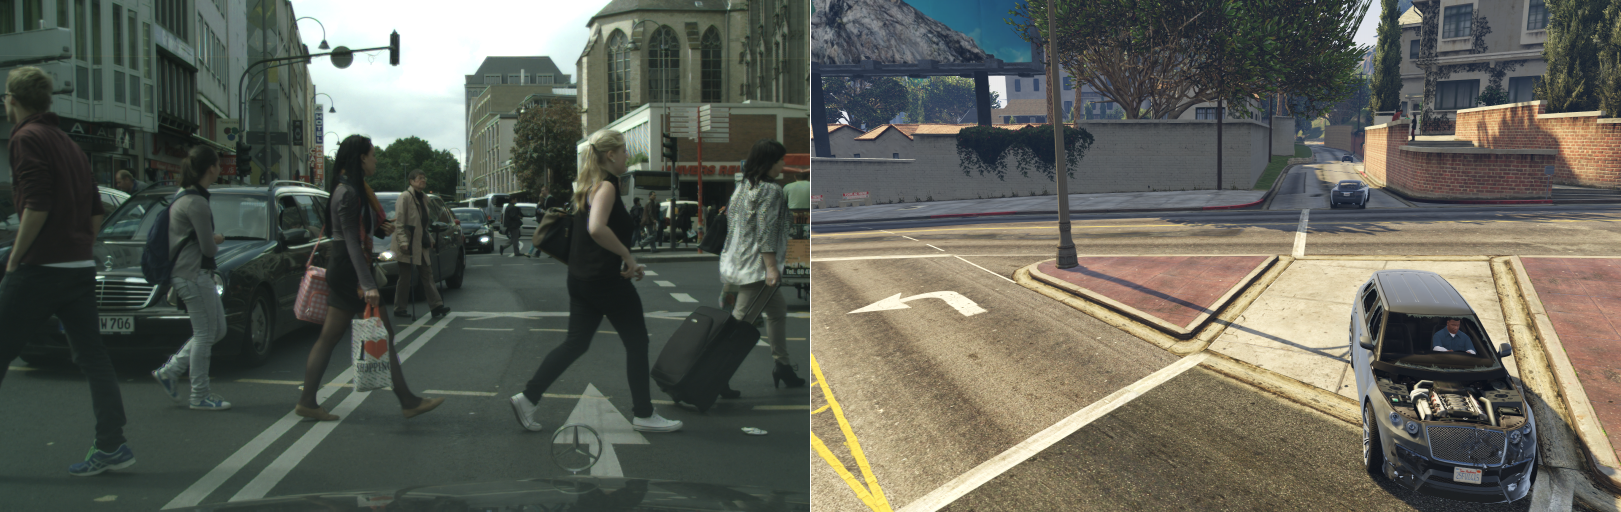
\includegraphics[width=0.8\textwidth]{../images/DA_examples_cityscapes_gta.png}
	\caption{Example images for the the two domains relevant for this work. A real image from the cityscapes dataset \cite{Cordts_2016_CVPR} (left) and a synthetic image from the GTA5 dataset \cite{Richter_2016_ECCV} (right)}
	\label{fig:DA_examples}
\end{figure}

\section{Semantic Segmentation}
Semantic Segmentation is one of the most important aspects in autonomous driving. It is the task of semantically segmentating objects in an image, i.e. labeling each pixel according to what object it belongs to. See Figure \ref{fig:semseg} for examples.

\begin{figure}
	\centering
	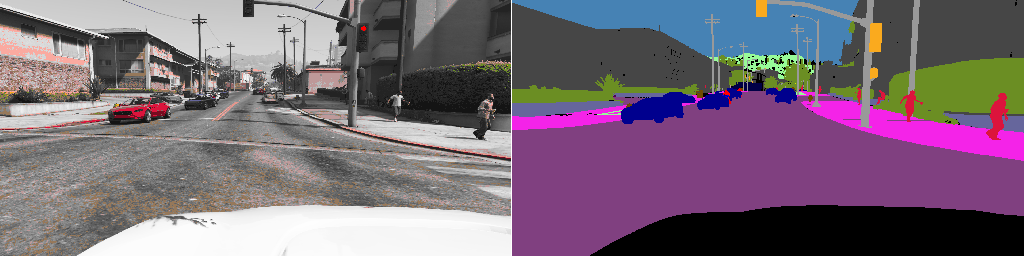
\includegraphics[width=\textwidth]{../images/semseg.png}
	\caption{Examples of a semantic segmentation images. Image taken from the GTA5 dataset \cite{Richter_2016_ECCV} (left) and same image mapped to Cityscapes Id values (pixel values 0-19, adapted to brighter values here to improve visibility). Streets in purple, sidewalks in pink, pedestrians red, cars, blue in the left image, which is mainly for visualization purposes. The right image is used for processing.}
	\label{fig:semseg}
\end{figure}



\section{Generative Adversarial Networks}
Generative Adversarial Networks (GANs) implement a two-player-game:\\
A Discriminator learns from a given data distribution what is ``real''. The Generator generates data. The goal of the generator is to fool the discriminator into believing the generated data is ``real'' i.e. tries to create samples coming from the same distribution as the ``real'' data. The discriminator will label anything as ``fake'' that doesn't resemble the learned ``real'' data distribution. This can be described as a 2 classes classification, with classes real and fake). This way GANs can learn to generate realistically looking images of faces, translate images of art from one style to another and improve semantic segmentation.
The generative model generally uses \textit{maximum likelihood estimation}. In \cite{DBLP:journals/corr/Goodfellow17} it is described in the following way:
\begin{quote}
	The basic idea of maximum likelihood is to define a model that provides an estimate of probability distribituion, parametereized by parameters $\theta$. We then refer to the \textbf{likelihood} as the probability that the model assigns to the training data: $\prod_{i=1}^{m}p_{\text{model}}(x^{(i)}; \theta)$
\end{quote}
The parameter $\theta$ that maximizes the likelihood of the data is better found in $\log$ space
\begin{align}
	\theta^* &= \underset{\theta}{\arg \max} \prod_{i = 1}^{m} p_{\text{model}} (x^{(i)}; \theta)\\
	&= \underset{\theta}{\arg \max} \log \prod_{i=1}^{m} p_{\text{model}}(x^{(i)}; \theta)\\
	&= \underset{\theta}{\arg \max} \sum_{i = 1}^{m} \log p_{\text{model}}(x^{(i)}; \theta)
\end{align}
as the maximum of the function is at the same $\theta$ value and we now have a sum which aswell eliminates the possibility of having underflow by multiplying multiple very small probabilities together.
Formally GANs are a structured probabilistic model (more info: Chapter 16 of Goodfellow et al. 2016) containing latent variables z and observed variables x.
The generator is defined by a function G that takes $\mathbf{z}$ as input and uses $\theta^{(G)}$ as parameters, the discriminator by a function D that takes $\mathbf{x}$ as input and uses $\theta^{(D)}$ as parameters. Both players have cost functions that are defined in terms of both players' parameters. The discriminator  wishes to minimize $J^{(D)}(\theta^{(D)}, \theta^{(G)})$ and must do so by controlling only $\theta^{(D)}$. This is analogous for the generator: he tries to minimize $J^{(G)}(\theta^{(D)}, \theta^{(G)})$ while controlling only $\theta^{(G)}$. In contrast to an optimization problem that has a solution that is the (local) minimum (a point in parameter space where all neighboring points have greater or equal cost), the GAN objective is a game. The solution to a game is a Nash equilibrium \cite{Nash48}, meaning that each player chooses the best possible option or strategy in respect to what the other player(s) choose. Here the Nash equilibrium is a tuple $(\theta^{(D)}, \theta^{(G)})$ that is a local minimum of $J^{(D)}$ with respect to $\theta^{(D)}$ and a local minimum $J^{(G)}$ with respect to $\theta^{(G)}$.
\textbf{The generator} is simply a differentiable function G. When $\mathbf{z}$ is sampled from some simple prior distribution, G(z) yields a sample of $\mathbf{x}$ drawn from $p_{\text{model}}$. Typically a deep neural network is used to represent G. \\
The game plays out in two scenarios. The first is where the discriminator D is given random training examples $\mathbf{x}$ from the training set. The goal of the discriminator here is for $D(\mathbf{x})$ to be near 1. In the second scenario, random noise $\mathbf{z}$ is input to the generator. The discriminator then receives input $G(\mathbf{z})$, a fake sample by the generator. The discriminator strives to make $D(G(\mathbf{z}))$ approach 0 while the generator tries to make that approach 1. The games Nash equilibrium corresponds to $G(\mathbf{z})$ being drawn from the same distribution as the training data. Under the assumption that the inputs to the discriminator are half real and half fake, this corresponds to $D(\mathbf{x}) = \frac{1}{2}$ for all $\mathbf{x}$.

\paragraph{Training}
On each step, two minibatches are sampled: a minibatch of $\mathbf{x}$ values from the dataset and one of random noise $\mathbf{z}$. Then two gradient steps are made simultaneously (simultaneous SGD): one updating $\theta^{(D)}$ to reduce $J^{(D)}$ and one updating $\theta^{(G)}$ to reduce $J^{(G)}$.

\paragraph{Cost functions} There are many different cost functions that can be used for GANs. See chapter \ref{sec:techniques} for the ones that the techniques in this work use.


\paragraph{Advantages and Disandvantages}
\paragraph{non-convergence} When training GANs, while updating one player so that he makes the best possible current move and goes downhill the loss curve it is possible that the counterfeit player gets updated into going uphill the loss curve. This is in contrast to optimization problems where one tries to find a (local) minimum of the loss curve for example through stochastic gradient decent (SGD). Because there is only one gradient instead of the two in GAN objectives, the model generally makes reliable downhill progress during training. The result is that GANs often oscillate in practice due to the nature of having two players playing against each other, each trying to achieve the optimal outcome for themselves.

\paragraph{mode collapse} occurs when the generator learns to map different inputs to the same output. This results in generated data that is missing diversity. A solution is proposed in \cite{DBLP:journals/corr/ZhuPIE17}: Using a batch history of 50 images so that the discriminator also learns the distribution of images of the training data and can therefore make sure that the generator will not generate the same small set of images. Partial mode collapse refers to scenarios in which the generator makes multiple images containing the same color or texture themes, or multiple images containing different views of the same dog. See Figure \ref{fig:mode_collapse} for an example.


\begin{figure}
	\centering
	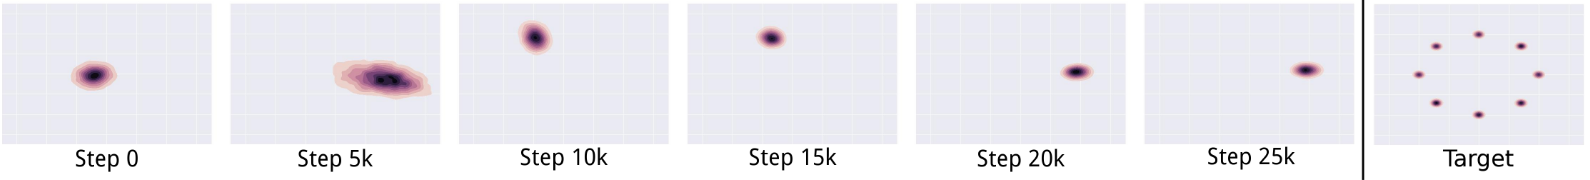
\includegraphics[width=\textwidth]{images/metz_et_al_mode_collapse.png}
	\caption{target data distribution of a toy dataset (right) and the data distribution of generated samples. Mind that the generated sample distribution hops from one mode to the next as the discriminator learns to recognize each mode as fake. Image from \cite{DBLP:journals/corr/MetzPPS16}}
	\label{fig:mode_collapse}
\end{figure}
\chapter{Related Work}
\label{sec:related_work}

This chapter will discuss the current state-of-the-art and related work on the topic of \textbf{Domain Adaptation}.


\section{Domain Adaptation for Structured Output via Discriminative Patch Representation}

see \cite{Tsai2019DomainAF}

\subsection{Abstract}
\begin{itemize}
	\item labeling data is expensive
	\item therefore propose domain adaptation method to adapt labeled source data to unlabeled target domain (e.g. GTA5 (playing for data) to city-scapes)
	\item learn discriminative feature representations of patches based on label histograms in the source domain, through construction of clustered space
	\item then use adversarial learning sscheme to push feature representations in target patches to the closer distributions in source ones
	\item can integrate a global alignment process with this patch-level alignment and achieve state-of-the-art performance on semantic segmentation
	\item extensive ablation studies on numerous benchmark datasets with various settings (e.g. synth-to-real, cross-city)
\end{itemize}

\subsection{Introduction}

\begin{itemize}
	\item pixel-level annotation of ground truth expensive. e.g. road-scene iamges of different cities may have various appearance distributions, differences over time and weather
	\item existing state-of-the-art methods use feature-level or output space adaptation, exploiut global distribution alignment, such as spatial layout, but these might differ significantly between two domains due to differences in camera poses or field of view
	\item authours instead match patches that are more likely to be shared across domains regardless of where they are located
	\item consider label histograms as a factor (Kulkarni et al., 2015; Odena et al., 2017) and learn discriminative representations for patches to relax high-variation problem among them
	\item use this to better align patches between source and target domains
	\item utilize two adversarial modules to align global/patch-level distributions
	\item global one based on output space adaptation (Tsai et al. 2018)
	\item take source domain labels and extract label histogram as a patch-level representation
	\item then apply K-means clustering to group extracted patch representations into $K$ clusters \todo{read this part again for better understanding (page 2)}
\end{itemize}

\subsection{domain adaptation for structured output}

\begin{itemize}
	\item given source and target images $I_s,I_t \in \mathbb{R}^{H \times W \times 3}$ and source labels $Y_s$, the goal is to align predicted output distribution $O_t$ of target data with source distribution $O_s$
	\item use loss function for supervised learning on source data to predict the structured output, adversarial loss is adopted to align the global distribution
	\item further incorporate classification loss in a clustered space to learn patch-level discriminative representations $F_s$ from source output distribution $O_s$. For target data another adversarial loss is used to align patch-level distributions between $F_s$ and $F_t$, where the goal is to push $F_t$ to be closer to distributon of $F_s$.
	\item objective function :
	\begin{align}
		\mathcal{L}_{\text{total}}(I_s, I_t, Y_s, \Gamma(Y_s)) = \mathcal{L}_s + \lambda_d \mathcal{L}_d + \lambda_{\text{adv}}^g \mathcal{L}_{\text{adv}}^g + \lambda_{\text{adv}}^l  \mathcal{L}_{\text{adv}}^l
	\end{align}
	where $\mathcal{L}_s$ and $\mathcal{L}_d$ are supervised loss function for learning structured prediction and discriminative representation on source data. $\Gamma$ denotes clustering process on ground truth label distribution. $\mathcal{L}_{\text{adv}}^g, \mathcal{L}_{\text{adv}}^l$ denote global and patch-level adversarial loss. $\lambda$'s are weights for the different loss function
	\item $\mathcal{L}_s$ can be optimized by fully-convolutional network $\mathbf{G}$ that predicts the structured output with the loss summed over the spatial map indexed with $h,w$ and number of categories $C$:
	\begin{align}
		\mathcal{L}_s(I_s, Y_s;\mathbf{G}) = - \sum_{h,w}\sum_{c \in C} Y_s^{(h,w,c)}\log(O_s^{(h,w,c)})
	\end{align}
	where $O_s = \mathbf{G}(I_s) \in (0,1)$ is the predicted output distribution through softmax function and is up-sampled to the size of the input image.
	\item with discriminator $\mathbf{D}_g$:
	\begin{align}
		\mathcal{L}_{\text{adv}}^g(I_s, I_t; \mathbf{G}, \mathbf{D}_g) = \sum_{h,w}\mathbb{E}[\log\mathbf{D}_g(O_s)^{(h,w,1)}] + \mathbb{E}[\log(1- \mathbf{D}_g(O_t)^{(h,w,1)})]
	\end{align}
	\item optimize following min-max problem with inputs dropped for simplicity:
	\begin{align}
		\underset{\mathbf{G}}{\min} ~ \underset{\mathbf{D}_g}{\max} \mathcal{L}_s(\mathbf{G}) + \lambda_{\text{adv}}^g \mathcal{L}_{\text{adv}}^g(\mathbf{G}, \mathbf{D}_g)
	\end{align}
	\item label histograms for patches: first randomly sample patches from source images, using a 2-by-2 grid on patches to extract spatial label histograms, and concatenate them into a vector, each histogram is a $2 \cdot 2 \cdot C$ dimensional vector. Second apply K-means clustering on these histograms, whereby the label for any patch can be assigned as the cluster center with the closest distance on the histogram
	\item add classification module $\mathbf{H}$ after the predicted output $O_s$, to simulate the procedure of constructin the label histogram and learn a discriminative representation\\
	learned representation: $F_s = \mathbf{H}(\mathbf{G}(I_s)) \in (0,1)^{U \times V \times K}$ (softmax function, $K$ is number of clusters)
	\item learning process to construct clustered space formulated as cross-entropy loss:
	\begin{align}
		\mathcal{L}_d(I_s, \Gamma(Y_s); \mathbf{G}, \mathbf{H}) = - \sum_{u,v} \sum_{k\in K} \Gamma(Y_s)^{(u,v,k)}\log(F_s^{(u,v,k)})
	\end{align}
	\item goal is now to align patches regardless of where they are located in the image (without spatial and neighborhood support)
	\item reshape $F$ by concatenating the $K$-dimensional vectors along the spatial map, results in $U \cdot V$ independent data points
	\item this reshaped data is denoted as $\hat{F}$, adversarial objective:
	\begin{align}
		\mathcal{L}_{\text{adv}}^l(I_s, I_t; \mathbf{G}, \mathbf{H}, \mathbf{D}_l) = \sum_{u,v}\mathbb{E}[\log \mathbf{D}_l(\hat{F}_s)^{(u,v,1)}] + \mathbb{E} [\log(1- \mathbf{D}_l(\hat{F}_t)^{(u,v,1)})]
	\end{align}
	where $\mathbf{D}_l$ is the discriminator to classify whether the feature representation $\hat{F}$ is from source or target domain
	\item integrate (3.5) and (3.6) into min-max problem in 3.4:
	\begin{align}
		\underset{\mathbf{G}, \mathbf{H}}{\min} ~ \underset{\mathbf{D}_g, \mathbf{D}_l}{\max} \mathcal{L}_s(\mathbf{G}) + \lambda_d \mathcal{L}_d (\mathbf{G}, \mathbf{H}) + \lambda_{\text{adv}}^g, \mathcal{L}_{\text{adv}}^g(\mathbf{G}, \mathbf{D}_g) + \lambda_{\text{adv}}^l \mathcal{L}_{\text{adv}}^l(\mathbf{G}, \mathbf{H}, \mathbf{D}_l)
	\end{align} 
\end{itemize}



\section{Effective Use of Synthetic Data for Urban Scene Semantic Segmentation}

see \cite{DBLP:journals/corr/abs-1807-06132}

\begin{itemize}
	\item foreground and background classes are not affected the same way by domain shifts
	\item foreground classes should be treated in a detection based manner as their shape looks natural even though their texture in synthetic images is not photo-realistic
	\item drawback of deep neural networks is need for massive amount of training data
	\item training on synthetic only makes models perform bad in the real world
	\item domain adaptation methods improve this but still require large sets of real images
	\item model cannot be trained off-line on synthetic data and work well when deployed into a new, real-world environment
	\item observation: not all classes suffer from the same type and degree of perceptual differences
	\item background texture looks more realistic than foreground, nevertheless foreground object shape look natural
	\item therefore should be treated differently
	\item use semantic segmentation on background classes because of texture realism
	\item use object detectors for foreground classes
	\item main discrimination between fore and background objects is shape
	\item trained seperately a DeepLab and Mask R-CNN \todo{cite} for object detection, followed by binary segmentation and class prediction, on synthetic data
	\item compare mIoU on foreground classes of Cityscapes
	\item outperforms semantic segmentation model on every class except \textit{motorcycle}
	\item from this observation: model that combines foreground masks produced by Mask R-CNN with pixel-wise predictions of DeepLab semantic segmentation network
	\item outperforms state-of-the-art domain adaptation techniques and can be further improved by making use of unsupervised real images
	\item \textbf{VEIS} (Virtual Environment for Instance Segmentation) proposed aswell, based on Unity3D
	\item automatically annotates synthetic images with instance-level segmentation for foreground classes
	\item when used with the proposed detector-based approach this data allows to boost semantic segmentation performance
\end{itemize}

\subsection{related work}

\begin{itemize}
	\item domain adaptation generally aims to reduce the gap between the feature distributions of the two domains (synthetic, real)
\end{itemize}

\subsection{Method}

\begin{itemize}
	\item use VGG16-based DeepLab model for background classes (with large field of view and dilated convolution layers)
	\item train on GTA5 dataset (background classes look photo-realistic)
	\item cross-entropy loss between network's predictions and ground-truth pixel-wise annotations of the sythetic images
	\item trained on fore- and background classes but foreground predictions are mostly discarded by the proposed approach
	\item use standard Mask R-CNN (object detection, binary mask extraction together with object classification) \todo{look at citation}
	\item fuse fore- and background predictions
	\item sort predicted segments according to confidence score, if current segment candidate overlaps with previous segment, pixels are removed in the overlapping region
	\item this yields a semantic segmentation map that only contains foreground classes and has large number of holes where no foreground object was found. Every pixel that is not already assigned to foreground class takes the label with highest probability at that pixel location in the DeepLab result
	\item remember: NO real data used during training of this method
	\item to extend approach for unsupervised training on real images: tread predictions of their method as pseudo ground truth for the real images. assign pixels that ware predicted as foreground classes by DeepLab model to an \textit{ignore} label, so that they are not used for training. 
\end{itemize}

\subsection{Implementation Details}
\begin{itemize}
	\item DeepLab: SGD, learning rate starting at $25 \times 10^{-5}$ with decrease factor of 10 every 40k iterations, momentum of 0.9, weight decy of 0.0005, mini-batches of size 1. weights initialized with those of VGG-16 classifier, pre-trained on ImageNet, due to limited GPU memory high resolution images were downsampled by a factor of 2 for training
	\item Mask R-CNN: implementation provided by Detectron framework \todo{cite}, train an end-to-end Mask R-CNN model with $64 \times $ 4d ResNeXt-101-FPN backbone, pre-trained on ImageNet, on the synthetic VEIS dataset. mini-batch of size 1, train model for 200k iterations, starting learning rate of 0.001, reducing to 0.0001 after 100k iterations
\end{itemize}


\section{Exemplar Guided Unsupervised Image-to-Image Translation with Semantic Consistency}

see \cite{DBLP:journals/corr/abs-1805-11145}

\begin{itemize}
	\item EGSC-IT network conditions the translation process on an exemplar image in the target domain
	\item assumption: image comprises of a content component shared across domains, and style component specific to each domain
	\item under guidance of exemplar from target domain apply Adaptive Instance Normalization to the shared content component, which allows to transfer the style information of the target domain to the source domain
	\item introduce feature masks that provide coarse semantic guidance without requiring the use of any semantic labels to avoid semantic inconsistencies during translation
	\item image-to-image (I2I) translation: task of mapping an image from a source domain to a target domain (e.g. semantic maps to real images, grey-scale to color, low-resolution to high-res)
	\item other approaches assume one-to-one mapping (e.g. cycleGAN) and fail to capture multimodal nature of image distribution within the target domain (many-to-many mapping, e.g. diffferent color and style of shoes in sketch-to-image translation, different seasons in syn2real street view translation)
	\item assume an image is composed of two disentangled representations: domain-shared representation that models the content in the image, second domain-specific representation that contains the style information
	\item unclear which style (time-of-day/season) to pick during image translation process, Isola et al. 2017 and Zhu et al. 2017b \todo{cite} show that using random noise for this can lead to mode collapse issues
	\item instead the image translation process is conditioned on arbitrary image in the target domain (i.e. an exemplar)
	\item like this EGSC-IT is enabled for multimodal (i.e. many-to-many) image translations, but also allows for explicit control over translation process depending on the exemplars used as guidance
	\item use weight sharing architecture proposed in UNIT (Liu et al. 2017 \todo{cite}), but instead of single latent space shared by both domains, a two component one is used (domain-shared component that contains semantic information (objects' category, shape, spacial layout), domain-specific style component that contains style information (texture, color)
	\item adaptive instance normalization (AdaIN) (Huang \& Belongie 2017 \todo{cite}) is applied to the shared content component of the source domain image using AdaIN parameters computed from the target domaoin exemplar
	\item directly applying AdaIN to the feature maps of the shared content component would mix up all objects and scenes in the image, making the image translation prone to failure when a n image contains diverse objects and scenes, therefore semantic labels as an additional form of supervision is used \todo{cite works that do this}. 
	\item instead of using data with labor-intensive annotations use computed feature masks
	\item feature masks: approximately decoupling different semantic categories in an unsupervised way under guidance of perceptual loss and adversarial loss
\end{itemize}

\subsection{Method}
\begin{itemize}
	\item weight sharing: to map image pairs (one from source domain, other target) to shared latent space, the last layer in the encoders ($E_A, E_B$) of the VAE-GAN and the first layer in the generators ($G_A, G_B$)  share their weights. (see \todo{cite UNIT, Liu et al. 2017})
	\item \todo{exemplar-based AdaIN for domain-specific style}
	\item \textit{Network architecture}: 1) two encoders $E_A, E_B$, each consisting of serveral strided convolutional layers and serveral residual blocks to compute the shared content component, 2) feature mask network and an AdaIN network, $F_A, F_B$ for $A \rightarrow B$ translation ($B \rightarrow A$ vise versa)have same architecture as the Encoder above \todo{above?} except for weight-sharing layers. 3) Two Generators, $G_A, G_B$, almost symmetric to the Encoders except that the up-sampling is done by transposed convolutional layers. 4) Two Discriminators, $D_A, D_B$ fully-convolutional networks containing a stack of convolutional layers. 5) A VGG sub-network (Simonyan \& Zisserman, 2015 \todo{cite}), VGG, that contains the first few layers (up to relu5\_1) of pre-trained VGG-19 (\todo{cite Simonyan \& Zisserman, 2015}), which is used to calculate perceptual losses. 
	\item Although UNIT is used as baseline framework, it can be replaced with any baseline framework with similar functionality
\end{itemize}

\subsection{Learning}
\begin{itemize}
	\item learning procedure of EGSC-IT contains VAEs, GANs, cycle-consistecy and perceptual losses.
	\item for more stable training, the feature mask network and AdaIN network gets pre-trained for each domain seperately within a VAE-GAN architecture, and use encoder part as fixed feature extractors ($F_A, F_B$) for the remaining training
	\item overall loss: 
	\begin{align}
		\mathcal{L}(E_A, G_A, D_A, E_B, G_B, D_B) &= \mathcal{L}_{\text{VAE}_\text{A}}(E_A, G_A) + \mathcal{L}_{\text{GAN}_{\text{A}}}(E_A,G_A,D_A) + \mathcal{L}_{\text{CC}_{\text{A}}}(E_A, G_A, E_B, G_B)\\
		&+  \mathcal{L}_{\text{VAE}_\text{B}}(E_B, G_B) + \mathcal{L}_{\text{GAN}_{\text{B}}}(E_B,G_B,D_B) + \mathcal{L}_{\text{CC}_{\text{B}}}(E_A, G_A, E_B, G_B)\\
		&+ \mathcal{L}_{\text{P}}(E_A, G_A, E_B, G_B)
	\end{align}
	\item VAEs, GANs and cycle-consistency losses identical to the ones used in \todo{cite Liu et al., 2017}
	\item \todo{add rest}
\end{itemize}

\subsection{Experiments}
\begin{itemize}
	\item translated between GTA5 and Berkeley Deep Drive (BDD) (\todo{cite both})
	\item Similar to FCN-score used by \todo{cite isola et al 2017} use the semantic segmentation performance to quantitatively evaluate the image translation quality
	\item first translate images from GTA5 dataset to arbitrary image in BDD
	\item only generate images of size $256 \times 512$ due to GPU memory limitations
	\item then train single-scale Deeplab model (\todo{cite Chen et al. 2018}) on the translated images and test it on BDD test set
	\item get mIoU scores
\end{itemize}

\subsection{Discussion}
since method doesn't use any semantic segmentation labels nor paired data, there are some artifacts in the results for some hard cases.\\
e.g. night $\rightarrow$ day translation more challenging than day $\rightarrow$ day, therefore sometimes hard for the model to understand semantics in such cases.\\
In the future it would be interesting to extend the method to semi-supervised setting to benefit from presence of some fully-labeled data

\section{Exploiting Semantics in Adversarial Training for Image-Level Domain Adaptation}

see \cite{DBLP:journals/corr/abs-1810-05852}

\begin{itemize}
	\item ResNet generator, U-Net discriminator
	\item 300k training iterations
	\item Adam optimizer, 0.0001 learning rate, batch size 2
	\item images cropped to 512x512
	\item images from GTA+annotations thereof, only images of cityscapes
\end{itemize}

\section{FCNs in the Wild: Pixel-level Adversarial and Constraint-based Adaptation}

see \cite{DBLP:journals/corr/HoffmanWYD16}

\begin{itemize}
	\item semantic segmentation is critical visual recognition task for a variety of applications ranging from autonomous agent tasks, such as robotic navigation and self-driving cars, to mapping and categorizing the natural world
	\item challenges when adapting between visual domains for classification: changes in appearance, lighting, pose
\end{itemize}


\subsection{work includes}
\begin{itemize}
	\item first unsupervised domain adaptation method for transferring semantic segmentation FCNs across image domains
	\item combination of global and local alignment methods, using global and category specific adaptation techniques
	\item align global statistics of source and target data using a convolutional domain adversarial training technique, using a novel extension of previous image-level classification approaches \todo{look up citations}
	\item given a domain aligned representation space, introduce generalizable constrained multiple instance loss function, which expands on weak label learning, but can be applied to the target domain without any extra annotations and explicitly transfers category layout information from a labeled source dataset
	\item use GTA5 and SYNTHIA + CityScapes datasets for synth2real
	\item cross season adaptation within SYNTHIA
	\item adaptation across real world cities
	\item perform detailed quantitative analysis of cross-city adaptation within CityScapes
	\item contribute BDDS (Berkeley Deep Driving Segmentation), unconstrained drive-cam dataset for semantic segmentation
	\item show Cityscapes to BDDS
	\item show that adaptation algorithm improves target semantic segmentation performance without any target annotations
\end{itemize}

\subsection{Related Work}

\begin{itemize}
	\item many recent approaches use fully convolutional networks (FCNs) for semantic segmentation, mapping input RGB space to semantic pixel space
	\item compelling because they allow direct end-to-end function that can be trained using back propagation
	\item original FCN formulation has been improved using dilated convolution (\todo{look at citation}) and post-processing techniques, such as Markov/conditional random fields
	\item high cost of collecting pixel level supervision motivates weak labels (typically image-level tags defining presence / absence of each class)
	\item Multiple instance learning (MIL) \todo{see citations}, reinforce confident predictions udring learning procecss
	\item improves method suggested by \todo{see citations} who use an EM algorithm to better model global properties of the images segments. Generalized by Pathak et al. who proposed a Constrained CNN, also able to model any linear constraints on the label space (i.e. presence / absence, percent cover)
	\item Hong et al. used auxiliary segmentation to generalize semantic segmentations to categories where only weak label information was available
	\item these methods all assume weak labels present during training time for both source and target domain
	\item authors consider strong supervision available in source domain, no supervision available in target domain
\end{itemize}

\subsubsection{Domain Adaptation}
\begin{itemize}
	\item domain adaptation in computer vision focuses largely on image classification, with much work dedicated to generalizing across domain shift between stock photographs of objects and the same objects photographed in the world
	\item recent work include \todo{some citations} which all learn a feature representation which encourages maximal confusion between the two domains
	\item other work \todo{cite }aims to align features by minimizing the distance between their distribtuions in the two domains
	\item based on GAN Liu et al. proposed coupled GAN to learn a joint distribution of images from both source and target datasets
	\item other computer vision task detection: Hoffmann et al., domain adaptation system: explicitly modeling the representation shift between classification and detection models, follow-up work which incorporated per-category adaptation using multiple instance learning. later converted into FCNs for evaluating semantic segmentation performance
\end{itemize}

\subsection{Fully Convolutional Adaptation Models}
\begin{itemize}
	\item source domain $S$, images $I_S$, labels $L_S$, trained source only model for semantic segmentation which produces pixel-wise per-category score map $\phi_S(I_S)$
	\item goal to learn semantic segmentation model which is adapted for use on unlabeled target domain $T$, images $I_T$, no annotations, parameters of such a network $\phi_T(\cdot)$
	\item if no domain shift: just apply source model directly to target domain
	\item however: commonly a difference between distribution of source labeled domain and target test domain
	\item therefore: \textit{unsupervised adaptation} approach
	\item first main shift: global changes may occur between two domains resulting in marginal distribution shift of corresponding feature space
	\item can occur in any domain, but most distinct in large domain shifts between very distinct domains (e.g. simulated and real domains)
	\item second main shift: due to category specific parameter changes. may result from individual categories having specific biases in the two domains (e.g. adapting between different cities: changes in appearance of signs and distribution of cars)
	\item propose unsupervised domain adaptation framework for adapting semantic segmentation models which directly tackles both the need for minimizing the global and the category specific shifts
	\item assumptions: source and target domain share same label space, source model achieves performance greater than chance on target domain
	\item introduce two new semantic segmentation loss objectives, one to minimize the global distribution distance, which operates over both source and target images, $\mathcal{L}_{\text{da}}(I_S, I_T)$, another to adapt category specific parameters using target images and transferring label statistics from source domain $P_{L_S}, \mathcal{L}_{\text{mi}}(I_T,P_{L_S})$
	\item to ensoure to not diverge too far from source solution, which is known to be effective for final semantic segmentation task, continue to optimize the standard supervised segnmentation objective on source domain $\mathcal{L}_{\text{seg}}(I_S, L_S)$
	\item goal: optimize joint objective:
	\begin{align}
		\mathcal{L}(I_S,L_S,I_T) &= \mathcal{L}_{\text{seg}}(I_S, L_S)\\
		&+ \mathcal{L}_{\text{da}}(I_S, I_T) + \mathcal{L}_{\text{mi}}(I_T,P_{L_S})
	\end{align}
	\item \todo{add illustration Figure 2}
	\item source domain data to update standard supervised loss objective, trained using source pixel-wise annotations
	\item both source and target data are used without any category annotations within fully-convolutional domain adversarial training to minimize global distance of feature space between the two domains
	\item category specific updates using a constrained pixel-wise multiple instance learning objective is performed on the target images, with source category statistics used to determine the constraints
	\item use front-end dilated FCN \todo{cite 33}, based on VGG16 \todo{cite 31} as base model
	\item 16 conv layers, last three conv layer converted from fully connected layers, called $f c_6, f c_7, f c_8$, followed by 8 times bilinear up-sample layer to produce segmentation in the same resolution as input images
\end{itemize}

\subsection{Global Domain Alignment}

\begin{itemize}
	\item recognition sought at pixel level, alignment of full image representations will marginalize out too much distribution information, limiting the alignment capability of the adversarial learning approach
	\item instead consider region corresponding to natural receptive field of each spatial unit in final representation layer (e.g. $fc_7$), as individual instances
	\item in doing so, the adversarial training procedure is supplied with the same information which is used to do final pixel prediction
	\item provides a more meaningful view of overall source and target pixel-space representation distribution distance which needs to be minimized
	\item ļet $\phi_{l-1}(\theta, I)$ denote output of last layer before pixel prediction according to network parameters $\theta$
	\item $\mathcal{L}_{\text{da}}(I_S, I_T)$ consists of alternating minimization objectives
	\item one concerning parameters $\theta$ of representation space, under which source and target distance $\min d(\phi_{l-1}(\theta, I_S), \phi_{l-1}(\theta, I_T))$ will be minimized for given distance function $d(\cdot)$.
	\item second: estimating distance function through training domain classifier to distinguish instances of source and target domains
	\item let $\theta_D$ domain classifier parameters
	\item learn domain classifier to recognize difference between source and target regions and use that classifier to guide distance iminimization of source and target representations
	\item let $\sigma (\cdot)$ denote softmax function, domain classifier predictions $p_{\theta_D}(x) = (\sigma(\phi(\theta_{D}, x)))$
	\item assuming output of layer $l-1$ has $H \times W$ spatial units, we can define domain classifier loss $\mathcal{L}_D$ as:
	\begin{align}
		\mathcal{L}_D = &- \sum_{I_S \in S} \sum_{h\in H}\sum_{w \in W} \log ( p_{\theta_D}(R^S_{hw}))\\
		&- \sum_{I_T \in T} \sum_{h\in H}\sum_{w \in W} \log (1 - p_{\theta_D}(R^T_{hw}))
	\end{align}
	where $R^S_{hw} = \phi_{l-1}(\theta, I_S)_{hw}$ and $R^T_{hw} = \phi_{l-1}(\theta, I_T)_{hw}$ denote source and target representation of each units, respectively
	\item inverse domain loss for convenience:
	\begin{align}
		\mathcal{L}_{\text{Dinv}} = &- \sum_{I_S \in S} \sum_{h\in H}\sum_{w \in W} \log (1 - p_{\theta_D}(R^S_{hw}))\\
		&- \sum_{I_T \in T} \sum_{h\in H}\sum_{w \in W} \log (p_{\theta_D}(R^T_{hw}))\\
	\end{align}
	\item alternating minimization procedure
	$$\begin{array}{cc}
		\underset{\theta_D}{\min} & \mathcal{L}_D\\
		\underset{\theta}{\min} &\frac{1}{2} [\mathcal{L}_D + \mathcal{L}_{\text{Dinv}}]
	\end{array}$$
	\item optimizing these two objectives iteratively amounts to learning the best possible domain classifier for relevant image regions and then using the loss of that domain classifier to inform the training of the image representations so as to minimize the distance between source and target domains
\end{itemize}

\subsection{Category Specific Adaptation}

\begin{itemize}
	\item \todo{cite 25 26?}
	\item compute by per image labeling statistics in source domain $P_{L_S}$. for each source image which contains class $c$, compute percentage of image pixels which have a ground truth label corresponding to this class. Can then compute histogram over these percentages and denote the lower $10\%$ boundary as $\alpha_c$, average values as $\delta_c$ and upper $10\%$ as $\gamma_c$
	\item use this to inform target domain size constraints, explicitly transferring scene layout information from source to target domain (e.g. street usually takes much more space in a autonomous driving image than signs).
	\item constrained MIL for the case where image-level labels are known: for a given target image for which a certain class $c$ is present, impose following constraints on output prediction map $p = \arg \max \phi (\theta, I_T)$
	\begin{align}
		\delta_c \leq \sum_{h,w} p_{hw}(c) \leq \gamma_c
	\end{align}
	\item encourages to not assign more pixels to class c than expected range observed in source domain
	\item optimize this objective with lower bound slack to allow for outlier cases wehre $c$ simply occupies less of the image than is average in source domain. Do not allow slack on upper bound constraint as it is important that no single class occupies too much of any given image
	\item general constraint: can be applied to all classes 
	\item optimize as in Pathak et al \todo{cite 25}
	\item modification: to prevent model diverging and over-fitting: use size constraint that if the lower $10\%$ of source class distribution $\alpha_c$ is greater than $0.1$, the down-weight the gradients due to these classes by factor of $0.1$. Can be viewed as re-sampling of the classes so as to come closer to a balanced set, allowing the relatively small classes potential to inform the learning objective
	\item need image-level labels for this approach, thus complete approach: predicting image-level labels, then optimizing for pixel predictions that satisfy the source transferred class size constraints. (e.g. source semantic segmentation yields: x pixels street, y pixels car, z pixels signs. target image-level labels are street and signs, make sure that semantic segmentation has at max x street and z sign classified pixels)
	\item \todo{reread last paragraph before experiments}
	\item given target image $I_T$, compute current output class prediction map $p = \arg \max \phi (\theta, I_T)$
	\item for each class comput percentage of pixels assigned to it in current prediction $d_c = \frac{1}{H\cdot W} \sum_{h\in H} \sum_{w\in W}(p_{hw} = c)$
	\item assign image-level label to class $c$ if $d_c > 0.1 \cdot \alpha_c$ (i.e. if currently labeling at least as many pixels as $10\%$ of the expected number for a true class appearing in the image)
\end{itemize}

\subsection{Experiments}
	domain adaptation tasks:
\begin{itemize}
	\item cities2cities
	\item season2season
	\item synth2real
	\item use front-end dilated FCN (\todo{cite 33}) as both the initialization for our method and as baseline model for comparison
	\item all code and models trained and evaluated in the Caffe (\todo{cite 16}) framework, available before camera-ready
	\item use IoU
	\item for c2c and syn2r follow evaluation protocol of \todo{cite 3} and train models with 19 semantic labels of Cityscapes
	\item for s2s use 13 semantic labels of SYNTHIA instead
\end{itemize}

\subsection{Datasets}

\subsubsection{Cityscapes}
\begin{itemize}
	\item 34 categories
	\item high resolution $2048 \times 1024$
	\item three parts: 2975 training samples, 500 validation samples, 1525 test samples
	\item split into european cities, different geographic and population distributions
\end{itemize}

\subsubsection{SYNTHIA}
\begin{itemize}
	\item 13 classes with different scenarios and sub-conditions
	\item for season to season use SYNTHIA-VIDEO-SEQUENCES, different cities, seasons, weathers, illumination, captured by 8 RGB cameras 360$^{\circ}$ visual field, use only dash-cam for this paper
	\item for synth2real use SYNTHIA-RAND-CITYSCAPES, 9000 random images from all sequences with Cityscapes-compatible annotations, as source domain data
\end{itemize}

\subsubsection{GTA5}
\begin{itemize}
	\item 24966 high quality labeled frames from realistic open-world computer game Grand Theft Auto V (GTA5)
	\item frames with $1914 \times 1052$ generated from fictional city Los Santos based on Los Angeles, CA.
	\item use whole dataset with labels compatible to Cityscapes categories for synth2real adaptation
\end{itemize}

\subsubsection{BDDS}
\begin{itemize}
	\item thousands of densely annotated dashcam video frames, hundreds of thousands of unlabeled frames
	\item $1280 \times 720$, 34 categories compatible to Cityscapes label space
	\item majority of data from New York and San Francisco (representative for eastern and western coasts)
	\item different from other existing driving dataset covers more challenging conditions (urban streetview at night, highway scene in rain,..)
\end{itemize}

\subsection{Quantitative and Qualitative Results}
\begin{itemize}
	\item first large distribution shift (synth2real)
	\item then medium shift (season2season)
	\item small shift (city2city in Cityscapes)
\end{itemize}


\todo{add import table contents}

\subsubsection{Large Shift: Synthetic to Real Adaptation}
\begin{itemize}
	\item for GTA to Cityscapes: compared to performance of source dilation model the domain adversarial training contributes $4.4\%$ raw and $\sim 20\%$ relative percentage mIoU improvement and multiple instance loss another $1.6\%$ raw and $\sim 6 \%$ relative
	\item for SYNTHIA to Cityscapes also measurable improvement
	\item raw $0.9\%$ for adversarial, raw $1.5\%$ with additional multiple instance loss
\end{itemize}

\subsubsection{Medium Shift: Cross Seasons Adaptation}
\begin{itemize}
	\item SYNTHIA season2season
	\item on average $\sim 3 \%$ mIoU improvement. Higher mIoU for 12/13 categories
	\item no improvement on class \textit{car} (probably because cars have little to no change in appearance through seasons in SYNTHIA)
	\item largest performance improvements through this method on categories like \textit{road} in shift from fall to winter
\end{itemize}

\subsubsection{Small Shift: Cross City Adaptation}
\begin{itemize}
	\item raw $3.6\%$ mIoU improvement through domain adversarial training, only $0.1\%$ through multiple instance loss
	\item only noticeable improvement from category specific alignment on \textit{traffic light, rider, train}, probably because domain shift between train and val sets mainly results from change in global appearance due to difference in city, specific category appearance may not change significantly though
\end{itemize}

\subsection{BDDS Adaptation}
\todo{find quantitative results}



\section{From Virtual to Real World Visual Perception using Domain Adaptation - The DPM Example}

see \cite{DBLP:journals/corr/LopezXGVR16}

\subsection{Need for Virtual Worlds}
\begin{itemize}
	\item in general best performing machine learning algorithms are \textit{supervised} i.e requiring annotated information (ground truth) for training
	\item human annotators (e.g. Amazon Mechanical Turk, LabelMe \todo{cite 48 and 53}) used for semantic segmentation but can't for pixel-wise optical flow and depth
	\item many deep CNNs developed today rely on an ImageNet pre-trained deep CNN which is modified or fine-tuned to solve a new task or operate in a new domain
	\item key for success of research community are powerful GPU hardware and large dataset with ground truth
\end{itemize}

\subsection{Need for Domain Adaptation}
\begin{itemize}
	\item problem of domain adaptation is not just a virtual-to-real issue but rather a sensor-to-sensor or environment-to-environment one \todo{cite 70, 71}
	\item \todo{deformable part-based model DPM 17}
	\item \todo{HOG+LPB/Linear-SVM paradigm 68, Haar+EOH/AdaBoost 69}
\end{itemize}

\subsection{Domain Adaptation for DPM in a Nutshell}
\begin{itemize}
	\item \todo{revisit this later if necessary}
\end{itemize}


\newpage

\section{Semantic-aware Grad-GAN for Virtual-to-Real Urban Scene Adaption}

see \cite{DBLP:journals/corr/abs-1801-01726}

\subsection{Introduction}
\begin{itemize}
	\item two main contributions: 
		\begin{enumerate}
			\item gradient-sensitive objective, emphasizes the semantic boundary consistencies between virtual images and adapted images. able to regularize the generator render distinct color/texture for each semantic region in order to keep semantic boundaries, which can alleviate the common blurry issues
			\item previous work often learn a whole image discriminator, makes pixels in image easily collapse into a monotonous pattern. appearance distributions for each semantic region should be regarded differently and purposely (e.g. road: coarse texture of asphalt concrete, vehicle: smooth and reflective)
		\end{enumerate}
	\item semantic-aware discriminator learns distinct discriminate parameters for examining regions with respect to each semantic label
	\item SG-GAN controllable architecture that personalizes texture rendering for different semantic regions and results in adapted images with finer details
\end{itemize}

\subsection{Related Work}
\subsubsection{Real-world vs. virtual-world data acquiring}
\begin{itemize}
	\item -
\end{itemize}
\subsubsection{Domain adaptation}
\begin{itemize}
	\item either by adapting scene images or adapting hidden feature representations guided by the targets
	\item Image-based adaption (aka image-to-image translation) can be summarized into two directions:
	\begin{enumerate}
		\item generated through feature matching (e.g. \todo{cite Gatys et al. 10}: combine content of one with style of other images through matching Gram matrix on deep feature maps, at expense of loss of some content information)
		\item GAN (e.g. \todo{Isola et al. 21} conditional GANs with mapping function for paired data, for unpaired data e.g. regularization term \todo{cite following} 37, cycle structure 24 45 47, weight sharing 29 30)
	\end{enumerate}
	\item some make use of both feature matching and adversarial training (5, 44)
	\item challenge: existing approaches often modify semantic information, e.g. sky adapted to tree structure or road lamp rendered from nothing
	\item hidden feature based adaption aims at adapting learned models to target domain (\todo{multiple citations}), by sharing weight (12) or incorporating adversarial discriminative setting (39), those mitigate performance degradation caused by domain shifting
	\item feature based adaption methods require different objectives or architecture for different vision tasks, thus not as widely applicable as image-based adaption
\end{itemize}

\subsection{Semantic-aware Grad-GAN}

\subsubsection{Semantic-aware cycle objective}
\begin{itemize}
	\item based on cycle-structured GAN objective
	\item unpaired images from virtual-world domain $V$ and real-world domain $R$ as $\{v\}^N_{i=1} \in V$ and $\{r\}^M_{i=1} \in R$
	\item SG-GAN learns symmetric mappings $G_{V\rightarrow R}$ and $G_{R\Rightarrow V}$ alogn with corresponding semantic-aware discriminators $SD_R, SD_V$
	\item $SD_R$ distinguishes between real-world images $\{r\}$ and fake real-world images $\{G_{V\rightarrow R}(v)\}$ and vice versa for $SD_V$
\end{itemize}

\subsubsection{Adversarial loss}

\begin{itemize}
	\item two sets of adversial losses applied to $(G_{V\Rightarrow R}, SD_R)$ and $(G_{R\Rightarrow V}, SD_V)$ pairs
	\item adversarial loss:
	\begin{align}
		\mathcal{L}_{\text{adv}}(G_{V\rightarrow R}, SD_R, V, R) &= \mathbb{E}_{r\sim p_{\text{data}}(r)}[\log SD_R(r)]\\
		&+ \mathbb{E}_{v\sim p_{\text{data}}(v)}[\log(1-SD_R(G_{V\rightarrow R}(v)))]
	\end{align}
	\item objective
	\begin{align}
		G^*_{V\rightarrow R} = \arg \underset{G_{V\rightarrow R}}{\min} \underset{SD_R}{\max} \mathcal{L}_{\text{adv}}(G_{V\rightarrow R}, SD_R, V, R)
	\end{align}
	\item analogous for other generator discriminator: $\mathcal{L}_{\text{adv}}(G_{R\rightarrow V}, SD_V, R, V)$
\end{itemize}

\subsubsection{Cycle consistency loss}
	\begin{align}
	\mathcal{L}_{\text{cyc}}(G_{V\rightarrow R}, G_{R\rightarrow V}, V, R) &= \mathbb{E}_{r\sim p_{\text{data}}(r)}[\lVert G_{V\rightarrow R}(G_{R\rightarrow V}(r)) - r \rVert_1]\\
	&+ \mathbb{E}_{v\sim p_{\text{data}}(v)}[\lVert G_{R\rightarrow V}(G_{V\rightarrow R}(v)) - v \rVert_1]
\end{align}

\begin{itemize}
	\item can be seen as introduction of a regularization on positions of image elements
	\item moving positions of image components is not encouraged
	\item model only with cycle-consistency can still map sky to tree (not semantic aware)
\end{itemize}

\subsubsection{Soft gradient-sensitive objective}

\begin{itemize}
	\item motivation of gradient-sensitive loss: no matter how texture of semantic classes change, there should be some distinguishable visual difference at boundaries of semantic classes
	\item visual differences for adjacent pixels can be captured through convolving gradient filters upon the image
	\item typical choice of gradient filter is Sobel filter (\todo{cite 38}) as $\mathbf{C} = \{C_x, C_y\}$:
	$\begin{array}{cc}
		C_x = 
		\begin{pmatrix}
			-1 & 0 & 1\\
			-2 & 0 & 2\\
			-1 & 0 & 1
		\end{pmatrix},
		C_y = 
		\begin{pmatrix}
			1 & 2 & 1\\
			0 & 0 & 0\\
			-1 & -2 & -1
		\end{pmatrix}
	\end{array}$
	\item since focus is visual difference on semantic boundaries, a 0-1 mask is necessary that only has non-zero values on semantic boundaries
	\item such mask can be retrieved by convolving a gradient filter upon semantic labeling since it only has different adjacent values on semantic boundaries
	\item semantic labeling obtained by human annotation, segmentation models, computer graphics tools (\todo{cite})
	\item multiply convolved semantic labeling and convolved image element-wise, to only pay attention to visual differences on semantic boundaries
	\item for input image $v$ and corresponding semantic labeling $s_v$ since we desire $v$ and $G_{V\rightarrow R}(v)$ share the same semantic information, greadient-sensitive loss for image $v$ can be defined as follows with $C_i$ and $C_s$ gradient filters for image and semantic labeling, $*$ convolution, $\odot$ element-wise multiplication, $|\cdot|$ absolute value,
	$\lVert \cdot \rVert_1$ L1-norm, $sgn$ sign function:
	\begin{align}
		l_{\text{grad}}(v,s_v,(G_{V\rightarrow R})) &= \lVert(|(|C_i * v |-|C_i*G_{V\rightarrow R}(v)|)|)\\
		&\odot (\alpha \times |sgn(C_s*s_v)|+ \beta)\rVert_1\\
		&s.t.\quad \alpha + \beta = 1 \quad \alpha, \beta \geq 0
	\end{align}
	\item in practice we may hold belief that $v$ and $G_{V\rightarrow R}(v)$ share smiliar texture within semantic classes
	\item texture can be extracted from image gradient, therefore a soft gradient-sensitive loss for $v$ can be defined as following to represent such belief, in which $\beta$ controls how much belief we have on texture similarities
	\begin{align}
		l_{s-\text{grad}}(v, s_v, G_{V\rightarrow R}, \alpha, \beta) &= \lVert(|(|C_i*v|-|C_i*G_{V\rightarrow R}(v)|)|)\\
		&\odot (\alpha \times |sgn(C_s*s_v)|+\beta)\rVert_1\\
		&s.t. \quad \alpha + \beta = 1 \quad \alpha, \beta \geq 0
	\end{align}
	\item $S_V$ semantic labeling for $V$, $S_R$ for R. final objective for soft gradient-sensitive loss for single image:
	\begin{align}
		\mathcal{L}_{\text{grad}}(G_{V\rightarrow R}, G_{R\rightarrow V}, V, R, S_V, S_R, \alpha, \beta) &= \mathbb{E}_{r\sim p_{\text{data}}(r)}[l_{s-\text{grad}}(r,s_r, G_{R\rightarrow V}, \alpha, \beta)]\\
		&+ \mathbb{E}_{v\sim p_{\text{data}}(v)}[l_{s-\text{grad}}(v,s_v, G_{V\rightarrow R}, \alpha, \beta)]
	\end{align}
	\item full objective with $\lambda_c$, $\lambda_g$ controlling relative importance of cycle consistency and soft gradient-sensitive loss compared to adversarial loss:
	\begin{align}
		\mathcal{L}(G_{V\rightarrow R}, G_{R\rightarrow V}, SD_V, SD_R) &= \mathcal{L}_{\text{adv}}(G_{V\rightarrow R}, SD_R, V, R)\\
		&+ \mathcal{L}_{\text{adv}}(G_{R\rightarrow V}, SD_V, R, V)\\
		&+ \lambda_c \mathcal{L}_{\text{cyc}}(G_{V\rightarrow R}, G_{R\rightarrow V}, V, R)\\
		&+ \lambda_g \mathcal{L}_{\text{grad}}(G_{V\rightarrow R}, G_{R\rightarrow V}, V, R, S_V, S_R, \alpha, \beta)
	\end{align}
	\item optimization target:
	\begin{align}
		G^*_{V\rightarrow R}, G^*_{R\rightarrow V} &= \arg \underset{\substack{G_{V\rightarrow R}\\ G_{R\rightarrow V}}}{\min}~ \underset{\substack{SD_R\\SD_V}}{\max}\mathcal{L}(G_{V\rightarrow R}, G_{R\rightarrow V}, SD_V, SD_R)
	\end{align}
\end{itemize}

\subsection{Semantic-aware discriminator}
\begin{itemize}
	\item introduction of soft gradient-sensitive loss contributes to smoother textures and clearer semantic boundaries
	\item scene adaption also needs to retain higher-level semantic consistencies (e.g. tone goes dark cause real world less ilumination, but may only want roads to be darker without changing the sky or even making it lighter)
	\item inappropriate holistic scene adaption because of traditional discriminator judging realism image-wise, regardless of texture difference in semantic-aware manner
	\item semantic-aware discriminators $SD_V$, $SD_R$
	\item idea: create separate pipeline for each different semantic class in the discriminator
	\item can be achieved by transiting number of filters in last layer of standard discriminator to number of semantic classes, then applying semantic masks upon filter to let each of them focus on different semantic classes
	\item last ($k$-th) layer's feature map of standard discriminator is typically a tensor $\mathbf{T}_k$ with shape $(w_k, h_k, 1)$, where $w_k$ stands for width and $h_k$ stands for height
	\item $T_k$ then compared with an all-one or all-zero tensor to calculate adversarial objective
	\item in contrast semantic-aware discriminator will change $\mathbf{T}_k$ as a tensor with shape $(w_k, h_k,s)$ where $s$ is number of semantic classes
	\item then convert image's semantic labeling to one-hot style and resize to $(w_k, h_k)$ which will result in mask $M$ with shape $(w_k, h_k, s)$ and $\mathbf{M}_{ij} \in \{01\}$
	\item by multiplying $\mathbf{T}_k$ and $\mathbf{M}$ element-wise, each filter within $\mathbf{T}_k$ will only focus on one particular semantic class
	\item Finally, by summing up $\mathbf{T}_k$ along the last dimension, tensor with shape $(w_k, h_k, 1)$ will be acquired and adversarial objective can be calculated the same way as standard discriminator
\end{itemize}

\subsection{Experiments}

\subsection{Experiments - Implementation}

\subsubsection{Dataset}
\begin{itemize}
	\item randomyl sample 2k images from GTA5 dataset and Cityscapes training set as training images for $V$ and $R$.
	\item another 500 each for visual comparison and validation
	\item Cityscapes validation set will later be used to evaluate semantic segmentation scores
	\item trained on this, the model's name is \textbf{SG-GAN-2K}
	\item another training set on full GTA5 dataset and 2k Cityscapes images called \textbf{SG-GAN-25K}
\end{itemize}

\subsubsection{Network architecture}
\begin{itemize}
	\item use $256 \times 512$ images for training due to GPU memory limitation
	\item for generator adapt Isola et al. 21 (U-Net structure with skip connections between low and high level layers)
	\item for semantic-aware discriminator use variant of PatchGAN (21,47), which is a FCN consists of multiple layers (leaky-ReLU, instance norm (41), convolution) and helps discriminator identify realism patch-wise
\end{itemize}

\subsubsection{Training details}
\begin{itemize}
	\item to stabilize training use history of refined images (37) for training $SD_V$ and $SD_R$
	\item apply least square objective instead of log likelihood for adversarial loss, which is shown helpful in stabilizing training and generating higher quality images (Mao et al. 31)
	\item parameters in 3.32-3.35 set $\lambda_c = 10$, $\lambda_g = 5$, $(\alpha, \beta)$ as $(0,1)$ for first three epochs, then $(0.9, 1)$
	\item for gradient filters in 3.27-3.29 use Sobel Filter for $\mathbf{C}_i$ and filters 
	\begin{align}
		C_x = 
		\begin{pmatrix}
		0 & 0 & 0 \\
		-1 & 0 & 1\\
		0 & 0 & 0
		\end{pmatrix}
		,~
		C_y =
		\begin{pmatrix}
		0 & 1 & 0 \\
		0 & 0 & 0 \\
		0 & -1 & 0
		\end{pmatrix}
	\end{align}
	for $\mathbf{C}_s$ to avoid artifacts on image borders caused by reflect padding
	\item for number of semantic classes in discriminator cluster 30 classes (7) into 8 categories to avoid sparce classes i.e. $s = 8$
	\item learning rate 0.0002, batch size 1
	\item implemented based on TensorFlow framework (1) and train with single Nvidia GTX1080
\end{itemize}

\subsubsection{Testing}
\begin{itemize}
	\item semantic information only needed at training time
	\item at test time SG-GAN only requires images without semantic information
	\item since generators and discriminators are FCN, can handle high res $(1024 \times 2048)$ at test time
	\item test time 1.3 seconds/image with the GPU mentioned earlier
\end{itemize}

\subsection{Comparison with state-of-the-art methods}
\subsection{Comparison - Baselines}
\subsubsection{SimGAN}
\begin{itemize}
	\item (37)
	\item introduces self-regularization for GAN and local adversarial loss to train refiner for image adaption
	\item in experiments use channel-wise mean values as self-regularization term
	\item use architecture as proposed in 37
\end{itemize}

\subsubsection{CycleGAN}
\begin{itemize}
	\item (47) learns mapping functions through adversarial loss and cycle consistency loss
	\item uses ResNet (14) architecture for generators and PatchGAN (21) for discriminators
\end{itemize}

\subsubsection{DualGAN}
\begin{itemize}
	\item (45)
	\item uses U-Net structure for gen that are identical with SG-GAN
	\item PatchGAN as CycleGAN but follows loss format and training procedure of Wasserstein GAN (2)
\end{itemize}

\subsubsection{BiGAN}
\begin{itemize}
	\item (8,9) learns inverse mapping of standard GANs (13)
	\item standard GANs learn generators mapping random noises $Z$ to images $X$, i.e., $Z \rightarrow X$, BiGAN also aims at inferring latent noises based on images $X\rightarrow Z$
	\item By taking Z as image, BiGAN can also be used for unpaired scene adaption
	\item use code provided in (47)
\end{itemize}

\subsection{Comparison - Gualitative and quantitative evaluation}
\begin{itemize}
	\item generally SG-GAN generates better visualization results (clear boundaries, consistent semantic classes, smooth texture, etc.)
	\item SG-GAN2K shows its ability for personalized adaption (retains red color of vehicle's headlight but red color of sunset is changed to sunny yellow that is closer to real-world images)
	\item conduct A/B tests on AMT by comparing SG-GAN-2K and baseline apporaches pairwise
	\item 500 virtual-world images with $256 \times 512$ as input, present pairs of adapted images generated by different methods to workers for A/B tests
	\item for each image-image pair workers decide which is more realistic
	\item 123 workers participated 
	\item SG-GAN superiority over all other approaches by a high margin
	\item attribute that to clearer boundaries and smoother textures through soft gradient-sensitive loss, and personalized texture rendering with help of semantic-aware discriminator
\end{itemize}

\subsection{Ablation studies}
\subsubsection{Effectiveness of soft gradient-sensitive objective}
\begin{itemize}
	\item without: coarse semantic boundaries and rough textures
\end{itemize}

\subsubsection{.. of semantic-aware discriminator}
\begin{itemize}
	\item without SD lacks for details, e.g . color of traffic light, generates coarser textures, e.g. sky
\end{itemize}

\subsubsection{The effect of virtual training image size}
\begin{itemize}
	\item SG-GAN-25K slightly better than -2K
	\item improved performance may be only notable if dataset difference is in orders of magnitude
\end{itemize}

\subsubsection{Discussion}
\begin{itemize}
	\item very rare cases of unsatisfactory adaption results (e.g. tunnel scene where light looks like sunlight) due to lack of real world data for that situation while training
	\item investigating trade-off between annotation granularity and dataset size would be a possible next step
\end{itemize}

\subsection{Application on semantic segmentation}
\begin{itemize}
	\item train semantic segmentation model merely by adapted GTA5 dataset and evaluate on Cityscapes validation set
	\item for semantic segmentation model use architecture of Wu et al. 42 and exactly follow training procedure
	\item impressive results on Cityscapes \todo{tabel 2}
	\item SG-GAN $>$ CycleGAN
	\item further compared with hidden feature representation based adaption method proposed by Huffman et al. 18, achieves high performance margin
\end{itemize}

\section{Syn2Real: A New Benchmark for Synthetic-to-Real Visual Domain Adaptation}

see \cite{DBLP:journals/corr/abs-1806-09755}


\section{VisDA: The Visual Domain Adaptation Challenge}

see \cite{DBLP:journals/corr/abs-1710-06924}
\chapter{Domain Adaptation Techniques}
\label{sec:techniques}

\chapter{Experiments}
\label{sec:experiments}

In this chapter the three Domain Adaptation Techniques \textbf{CycleGAN} \cite{DBLP:journals/corr/ZhuPIE17}, \textbf{CyCADA} \cite{DBLP:journals/corr/abs-1711-03213} and \textbf{SG-GAN} \cite{DBLP:journals/corr/abs-1801-01726} will be compared by analysing similarities and differences. Furthermore, pre-trained models of each architecture were used to generate translated images on which a pre-trained DeepLabv3 \cite{DBLP:journals/corr/ChenPSA17} model then was used to perform semantic segmentation and the results will be compared on their Intersection over Union scores.

%\section{training the nets on tcml cluster} \todo{is this necessary or can we just use provided pre-trained models?}
%To train the models the tcml cluster of uni tübingen was used (\todo{add link to cluster website}). The cluster contains a lot of computing power with multiple compute nodes and a storage node. Each compute node has 4 CPUs and a NVidia 1080 Ti GPU and lots of RAM. In order to run the training code, it is necessary to create an .sbatch file. This file specifies how long a script needs to run, how much memory it needs and includes bash commands to run the script. Depending on what is specified in that .sbatch file the slurm manager system allocates ressources for that job and runs it as soon there are resources ready. While training cycleGAN mode collapse happened and the test images didn't get translated at all. Also to train for the 200 recommended epochs it would take around 2-3 weeks due to training taking a day for around 14 epochs. This is probably due to the fact that training cycleGAN is only possible on batches of size 1 which makes the vast resources available on the cluster not usable to their full potential. Also the student account can only run one job at once which makes it impossible to train different methods (cycleGAN, CyCADA, GradGAN) at the same time. Another issue is that it was not possible to visualize loss of generators and discriminators in order to supervise the training process and check if mode collapse or any other issue appeared. 

\section{Datasets}

\subsection{Synthetic dataset:\\
	Playing for Data: Ground Truth from Computer Games}

The GTA5 (Grand Theft Auto V) dataset is proposed in \cite{Richter_2016_ECCV}. It contains 24966 images taken from a street view in the game Grand Theft Auto V by Rockstar Games \cite{GTAV}. The images are provided with $1914 \times 1052$ pixels and are containing moving cars, objects, pedestrians, bikes, have changing lighting and weather conditions as well as day and night scenes. For all of these images the authors provide ground-truth semantic label maps that are compatible with the classes of the Cityscapes dataset \cite{Cordts_2016_CVPR}. Detouring, i.e. injecting a wrapper between the game and the graphics hardware to log function calls and reconstruct the 3D scene is used to create the images. This also enables a faster labeling process: Objects in a scene can be assigned an object ID through which assigned labels are propagated to other images containing this same object. Due to being more realistic than other existing synthetic street view datasets (e.g. SYNTHIA \cite{RosCVPR16}) the GTA5 dataset is very popular for training machine learning models related to autonomous driving. It therefore is used in this work. Example images and corresponding label maps are shown in Figure \ref{fig:p4d_examples} 


\begin{figure}
	\centering
	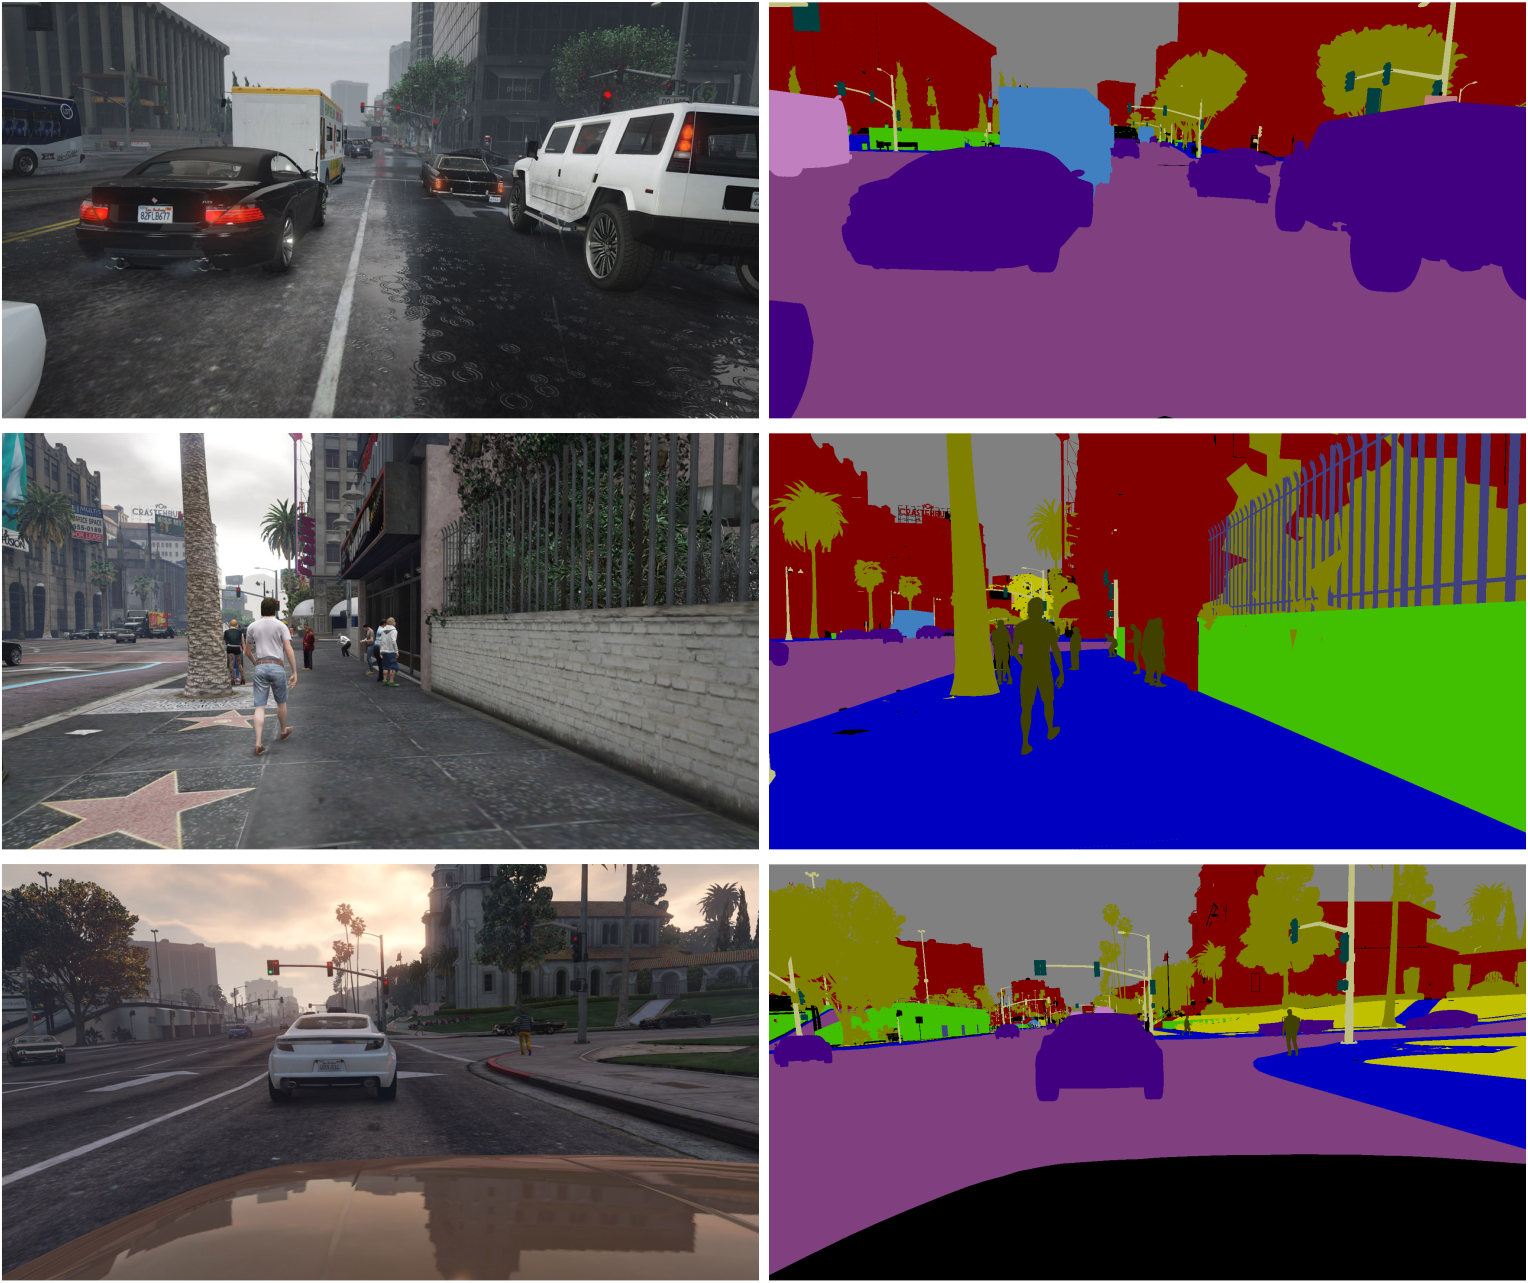
\includegraphics[width=\textwidth]{images/p4d_example.png}
	\caption{Example images (left) and corresponding ground-truth semantic label maps (right) provided in the GTA5 dataset \cite{Richter_2016_ECCV}.}
	\label{fig:p4d_examples}
\end{figure}

\newpage

\subsection{Real dataset:\\
	The Cityscapes Dataset for Semantic Urban Scene Understanding}

The Cityscapes dataset \cite{Cordts_2016_CVPR} is a large scale dataset containing car dashcam view images from 50 european cities. It includes 30 classes relevant for autonomous driving. The images include scenes in spring, summer and fall seasons and under different weather conditions. There are 5000 images provided together with fine annotations and 20000 together with coarse annotations. Due to the large amount of labeled data from a dashcam view and the inclusion of scenes with different weather and lighting conditions this dataset is often used to train deep neural networks that are related to autonomous driving. Due to the popularity and the GTA5 dataset containing compatible label maps, this work uses Cityscapes as the real dataset for the experiments. See Figure \ref{fig:cityscapes_examples} for Example images.

\begin{figure}
	\centering
	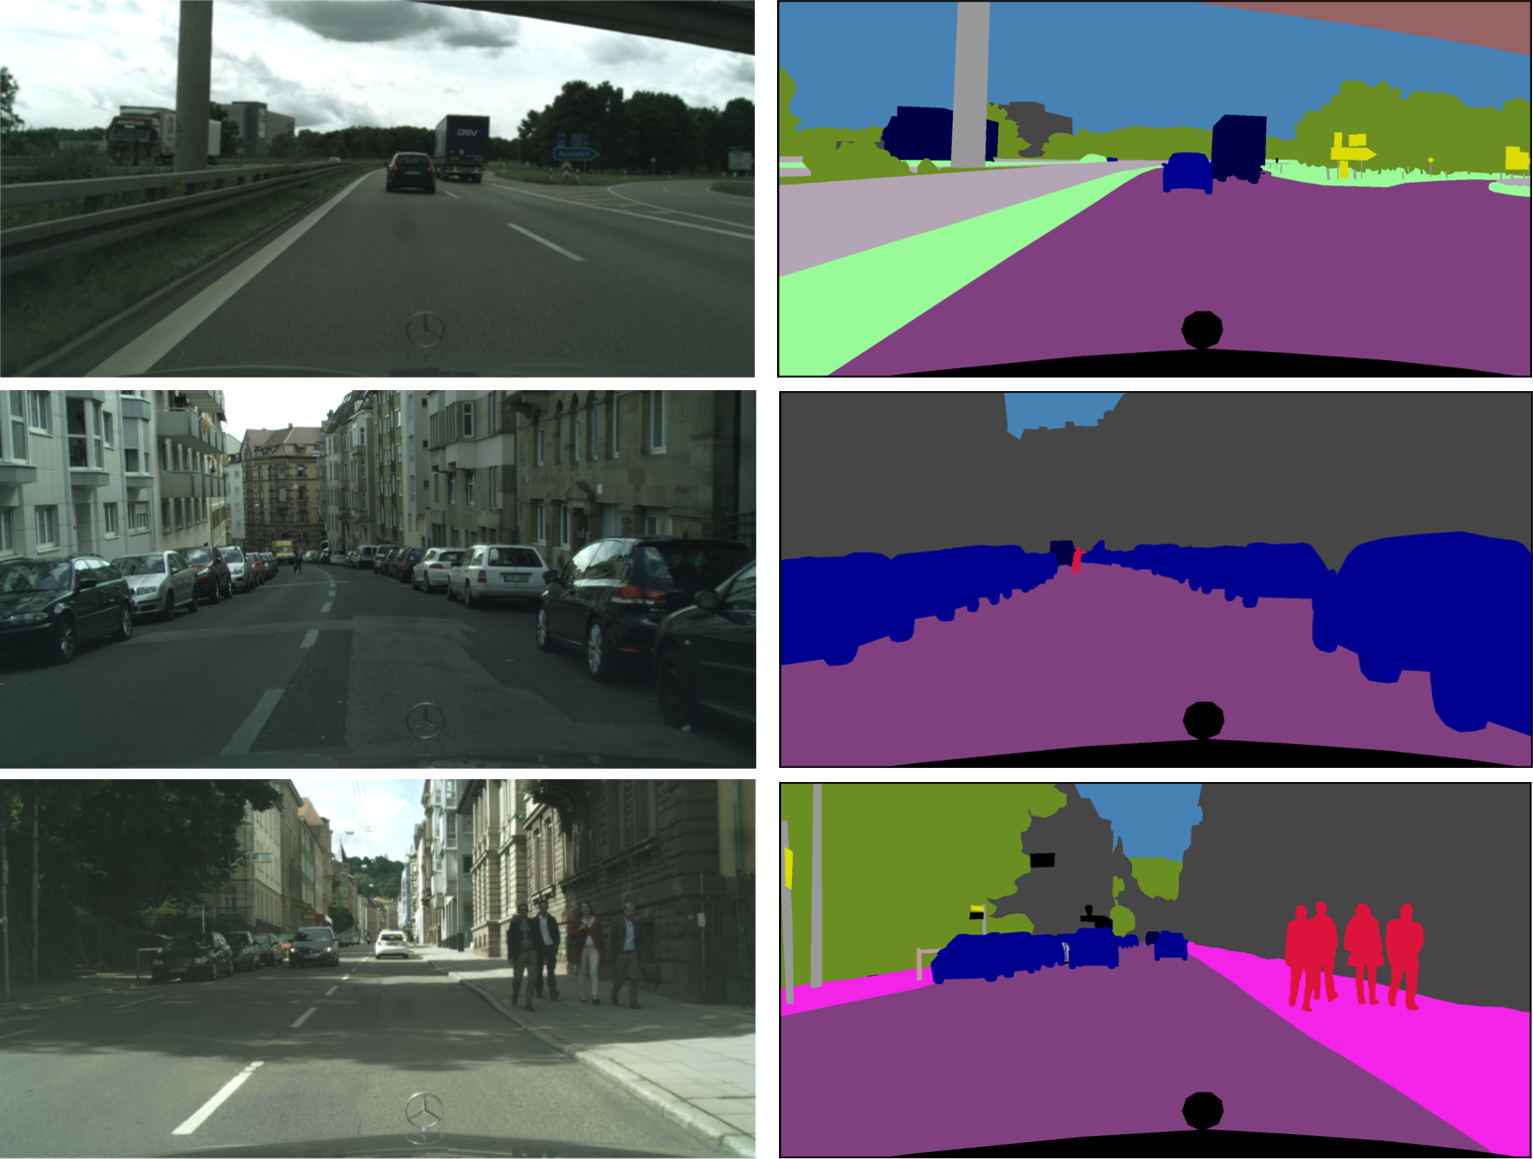
\includegraphics[width=\textwidth]{images/cityscapes_example.png}
	\caption{Example images (left) and corresponding ground-truth semantic label maps (right) provided in the Cityscapes dataset \cite{Cordts_2016_CVPR}.}
	\label{fig:cityscapes_examples}
\end{figure}

\section{Comparison Benchmark}
\subsection{Semantic Segmentation}
As this work is focused on datasets containing driving scenes the methods compared are applied to images that semantic segmentation will then be performed on. For the comparison Intersection over Union (IoU) is used. Intersection over Union is a metric often used to compare semantic segmentation methods' performance. All of the compared techniques were evaluated using IoU. It follows the following formula:
\begin{align*}
	\frac{\text{predicted pixels} \cap \text{ground truth pixels}}{\text{predicted pixels} \cup \text{ground truth pixels}}
\end{align*}
where predicted pixels are the pixels predicted for a specific class by the semantic segmentation model and ground truth pixels are the pixels containing the ground truth for that image. Usually, there are multiple different classes to predict and therefore it is common to calculate the mean IoU (mIoU) over all images that have predictions. To compare how well classes themselves are predicted by a model, one can also calculate the class IoU (cIoU).

\section{Methodology}
For the comparison each technique was used to translate a sample of 500 images from the GTA5 dataset to the Cityscapes domain. For CycleGAN and SG-GAN each, the authors provided pre-trained models. For CyCADA pre-translated images are provided in the project repository \cite{CyCADA}. To translate images with SG-GAN and CycleGAN the code provided in the repositories \cite{SG} and \cite{Cycle} was used. For the semantic segmentation task an implementation \cite{DLR} of DeepLabv3 \cite{DBLP:journals/corr/ChenPSA17} was used. To compute the IoU values the DeepLabv3 implementation uses the benchmark code provided by Cityscapes \cite{CSR}. All computations were run on a machine with Ubuntu 18.04 using an NVIDIA Geforce GTX 1070 with 8GB RAM. The images were scaled down to $512 \times 256$ pixels due to memory limitations while computing the CycleGAN samples.

\newpage

\section{Results}

\subsection{Quantitative}
As seen in Table \ref{table:results_quant}, CyCADA is the only method that improved average values for category and class semantic segmentation of the DeepLabv3 model. CyCADA improved the performance on a per category average compared to untranslated GTA5 data by $2.2\%$ points, CycleGAN decreased it by $2\%$ points and SG-GAN by $4.2\%$ points. While SG-GAN was only able to improve the ``nature'' category and CycleGAN additionaly improved flat as well, CyCADA was able to improve 4 of the 7 categories tested. For per class average values, CycleGAN and SG-GAN decreased performance by $2.6\%$ points and $1.1\%$ point, respectively while CyCADA improved it by $1.6\%$ points. For the per class comparison, CycleGAN improved performance for 7 of the 19 tested classes compared to untranslated GTA5. SG-GAN was able to improve the scores for 8 out of 19 classes while having the best values for ``bus'', ``building'', ``traffic sign'' and ``vegetation''. CyCADA improves performance for 10 classes while performing approximately the same as untranslated GTA5 images for ``vegetation''. It holds the top values for ``building'', ``fence'', ``motorcycle'', ``road'', ``terrain'', ``train'', ``truck'' and ``wall''. The biggest improvement for CyCADA is category ``train'' where it improves semantic segmentation accuracy by $25.5\%$ points compared to GTA5. See Table \ref{table:train} for an example that showcases the superior performance of semantic segmentation on the CyCADA translated image for the train category.

\begin{table}
	\centering
	\begin{tabular}{cc||c}
		\rotatebox[origin=c]{90}{\thead{GTA5 \\ (Ground Truth)}} & 
		\begin{minipage}[c]{0.45\textwidth}
			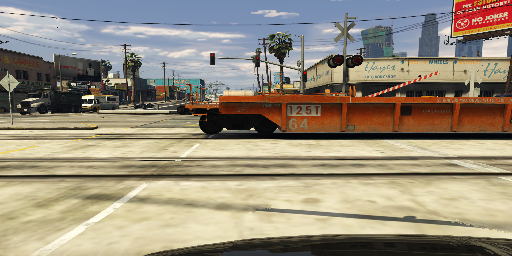
\includegraphics[width=\textwidth]{images/evaluation/GTA_gt_image_train.png}
		\end{minipage} & 
		\begin{minipage}[c]{0.45\textwidth}
			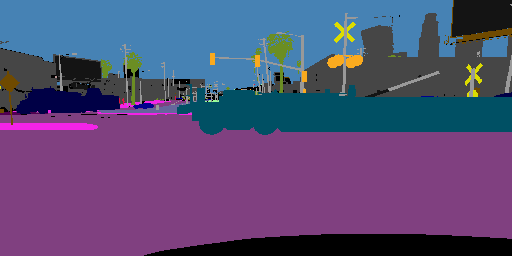
\includegraphics[width=\textwidth]{images/evaluation/GTA_gt_label_train.png}
		\end{minipage}\\
		\hline
		\hline
		\rotatebox[origin=c]{90}{GTA5} &
		\multicolumn{1}{c||}{} &
		\begin{minipage}[c]{0.45\textwidth}
			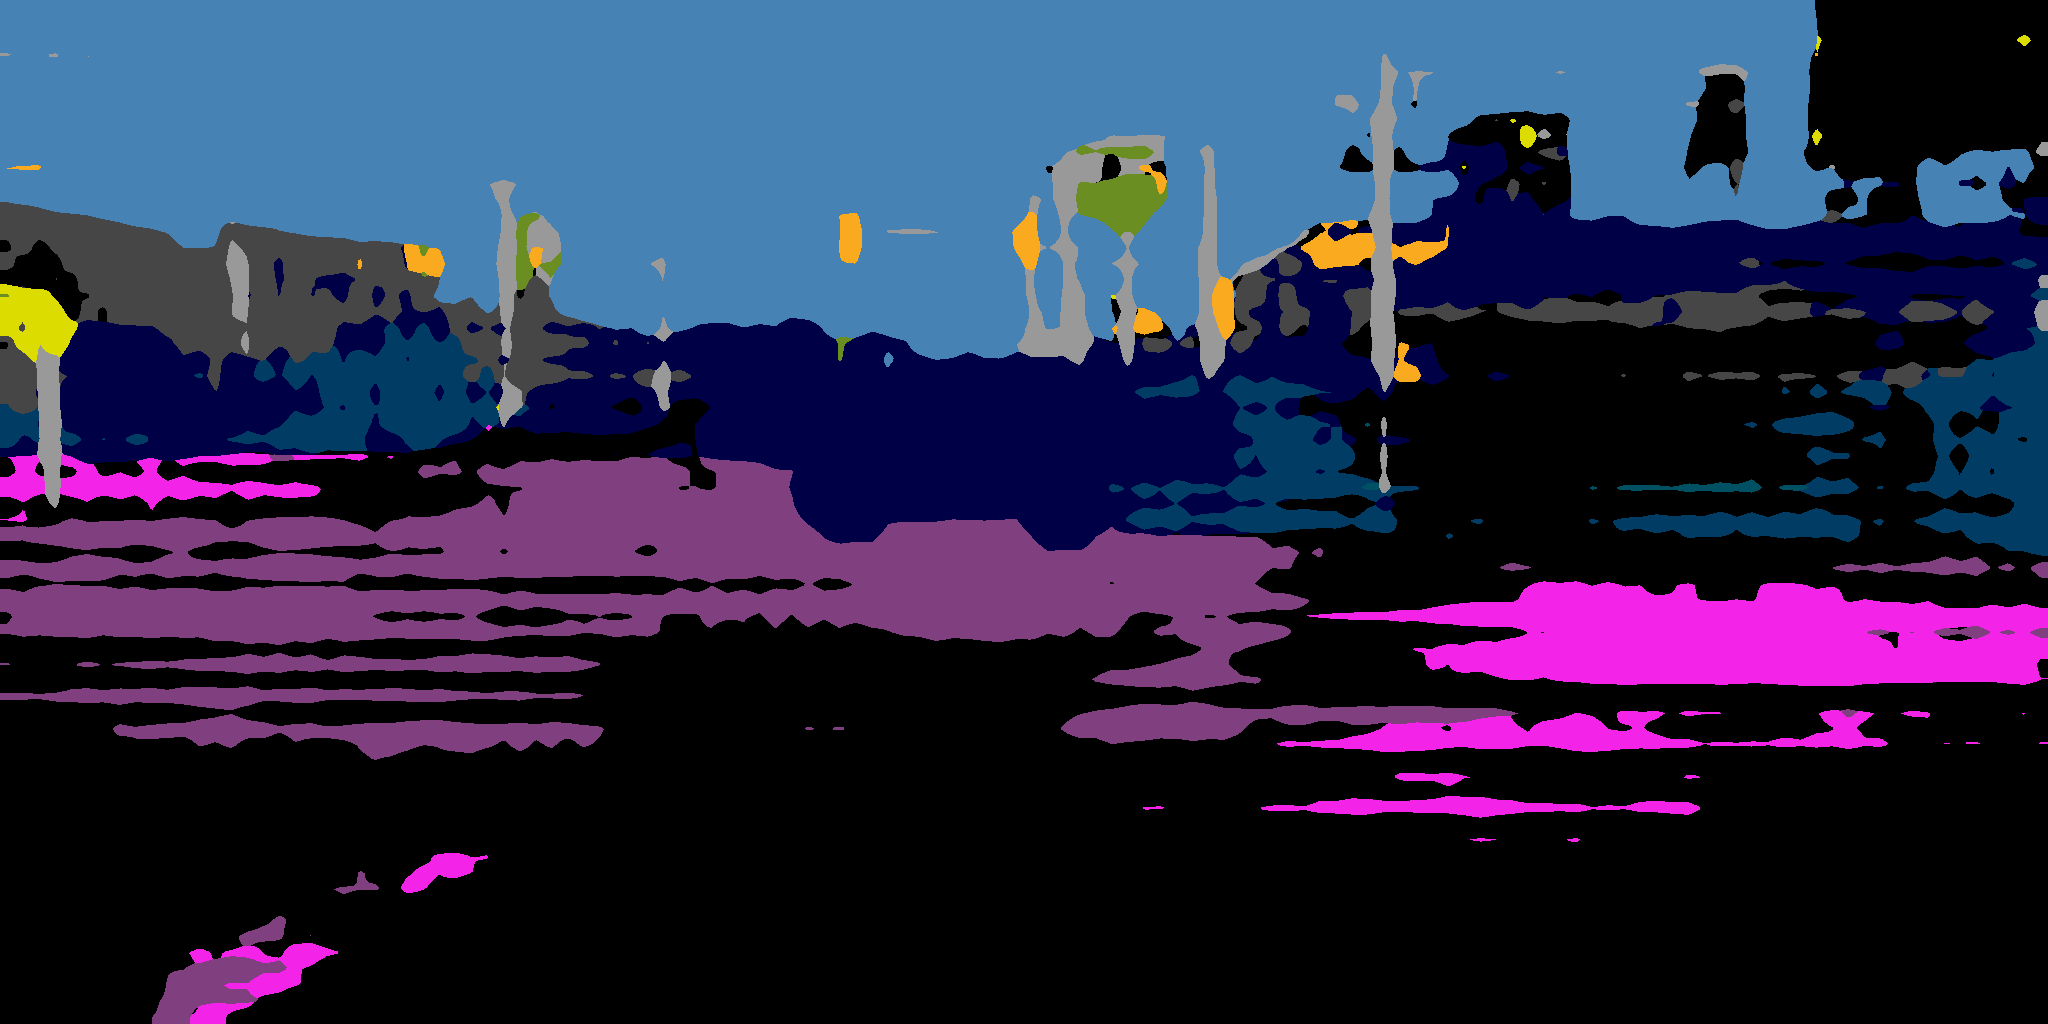
\includegraphics[width=\textwidth]{images/evaluation/GTA_pred_labels_train.png}
		\end{minipage}\\
		\rotatebox[origin=c]{90}{CycleGAN} &
		\begin{minipage}[c]{0.45\textwidth}
			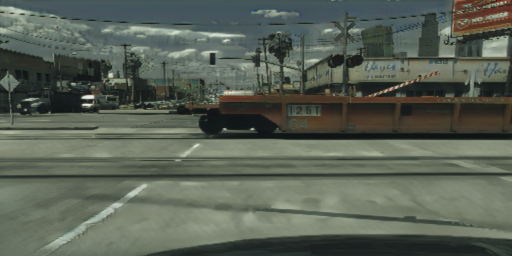
\includegraphics[width=\textwidth]{images/evaluation/CycleGAN_translated_train.png}
		\end{minipage} &
		\begin{minipage}[c]{0.45\textwidth}
			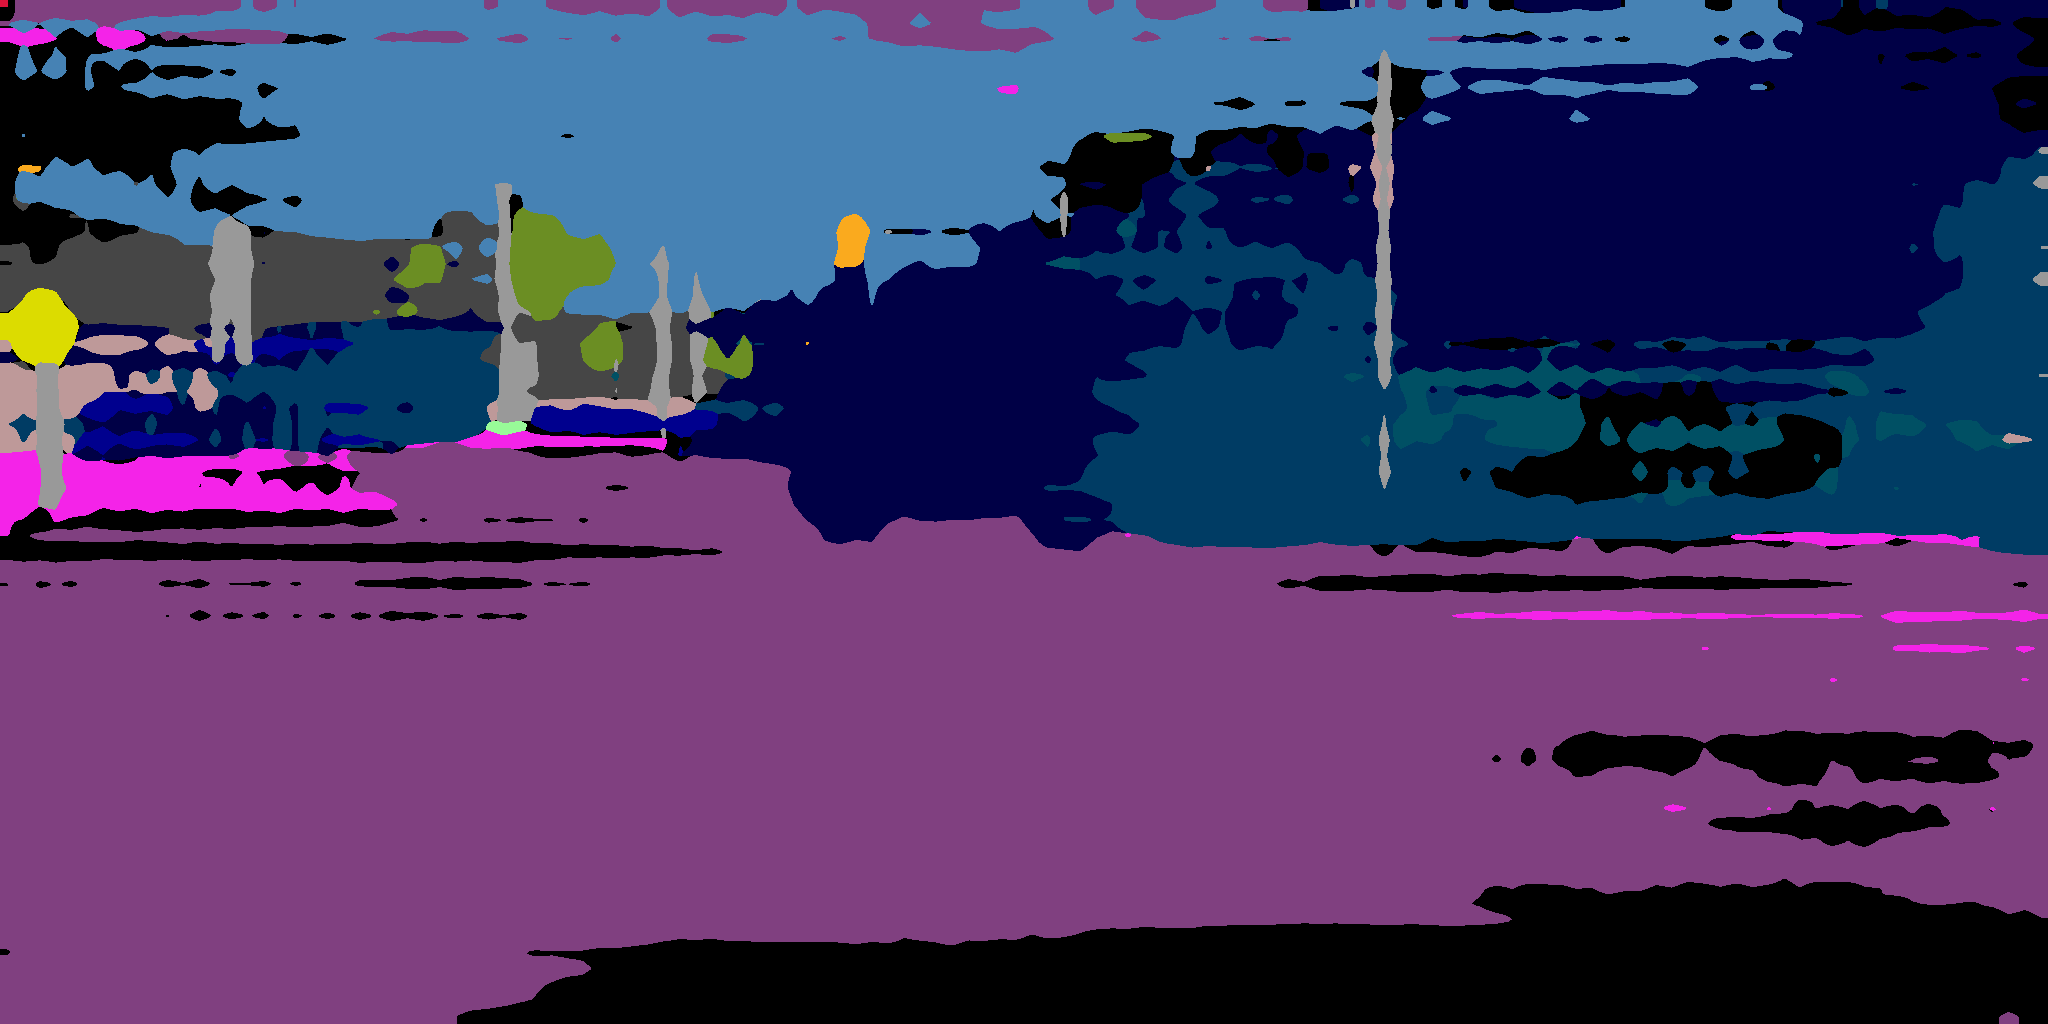
\includegraphics[width=\textwidth]{images/evaluation/CycleGAN_pred_labels_train.png}
		\end{minipage}\\
		\rotatebox[origin=c]{90}{CyCADA} &
		\begin{minipage}[c]{0.45\textwidth} 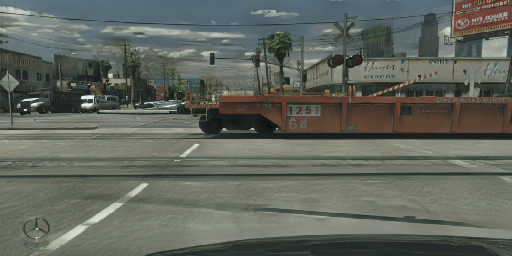
\includegraphics[width=\textwidth]{images/evaluation/CyCADA_translated_train.png} 
		\end{minipage}& 
		\begin{minipage}[c]{0.45\textwidth}
			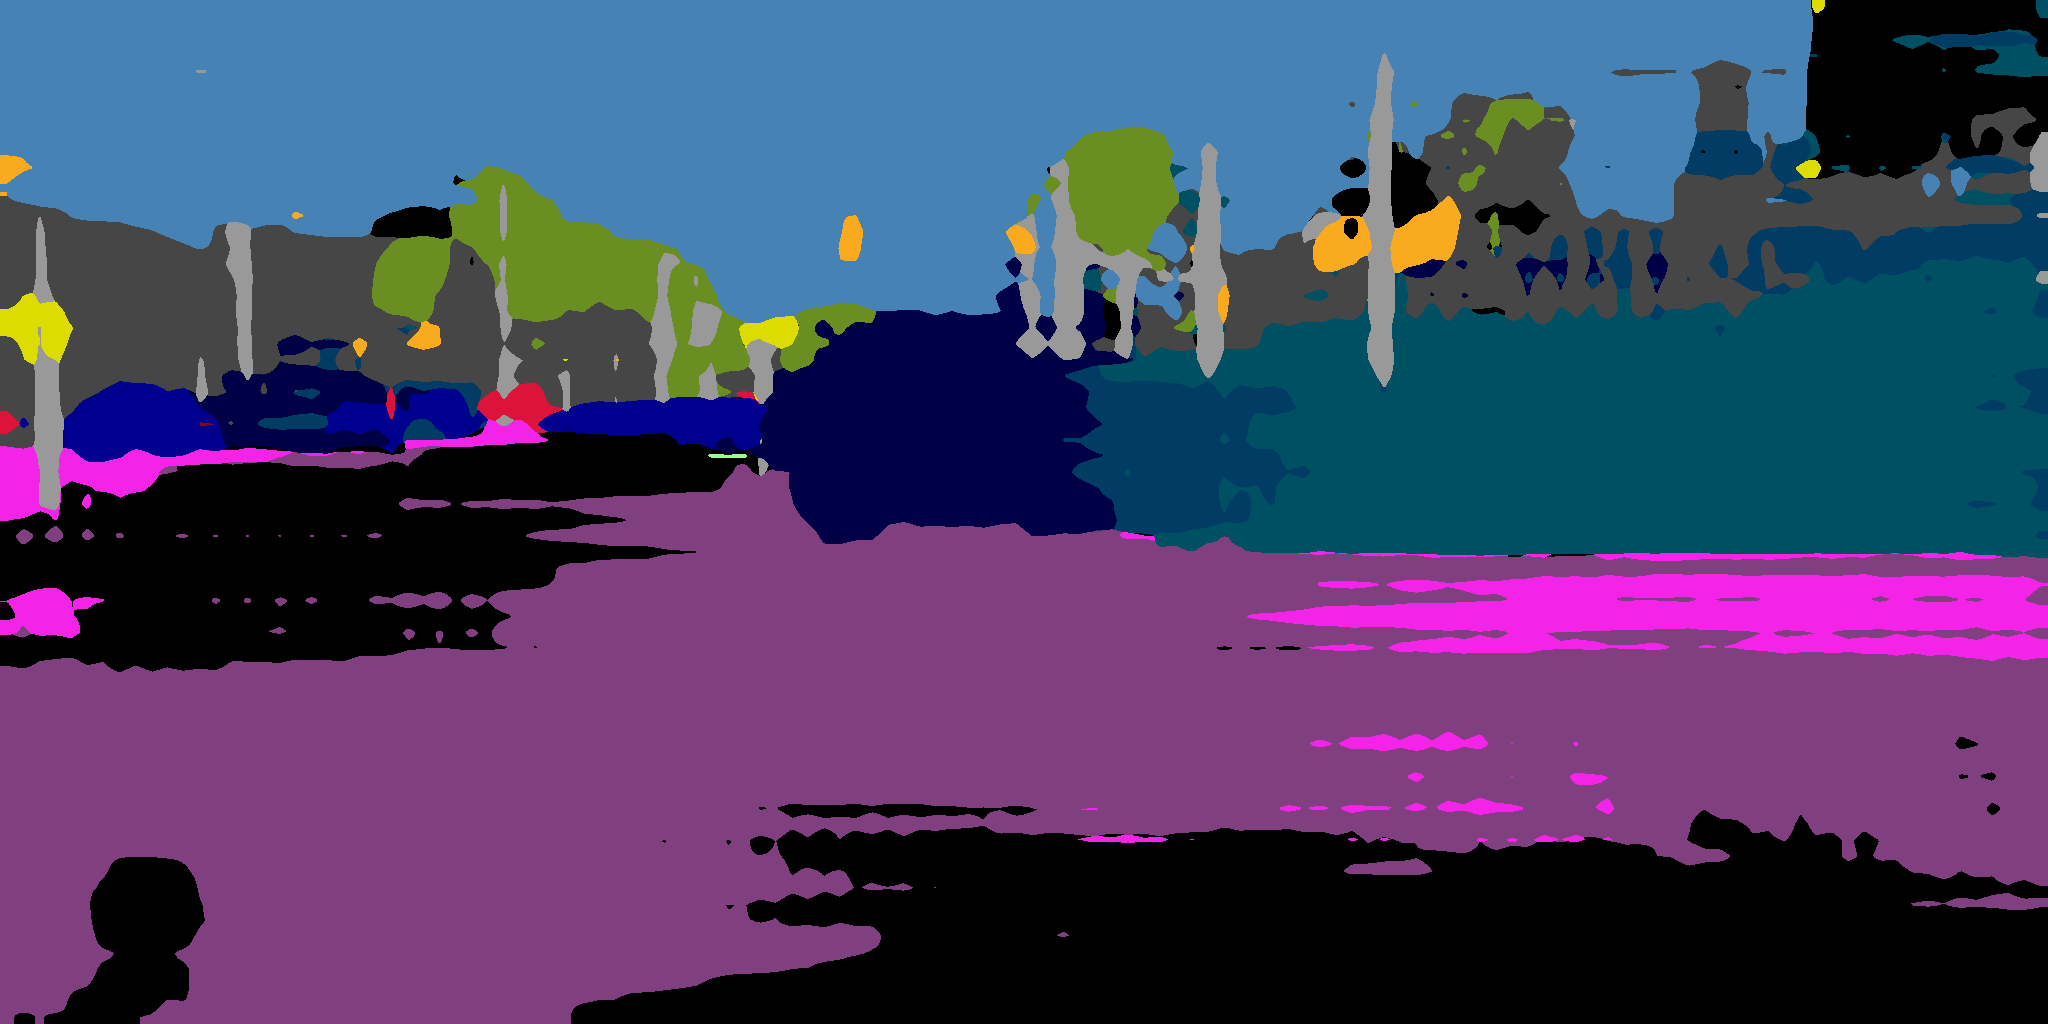
\includegraphics[width=\textwidth]{images/evaluation/CyCADA_pred_labels_train.png}
		\end{minipage}\\
		\rotatebox[origin=c]{90}{SG-GAN} &
		\begin{minipage}[c]{0.45\textwidth} 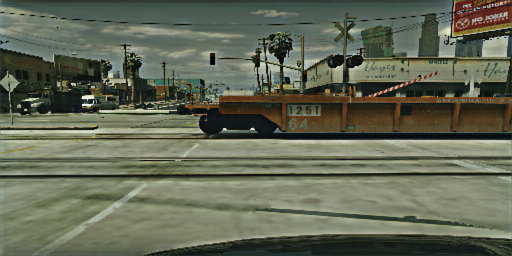
\includegraphics[width=\textwidth]{images/evaluation/SG-GAN_translated_train.png}
		\end{minipage} & 
		\begin{minipage}[c]{0.45\textwidth}
			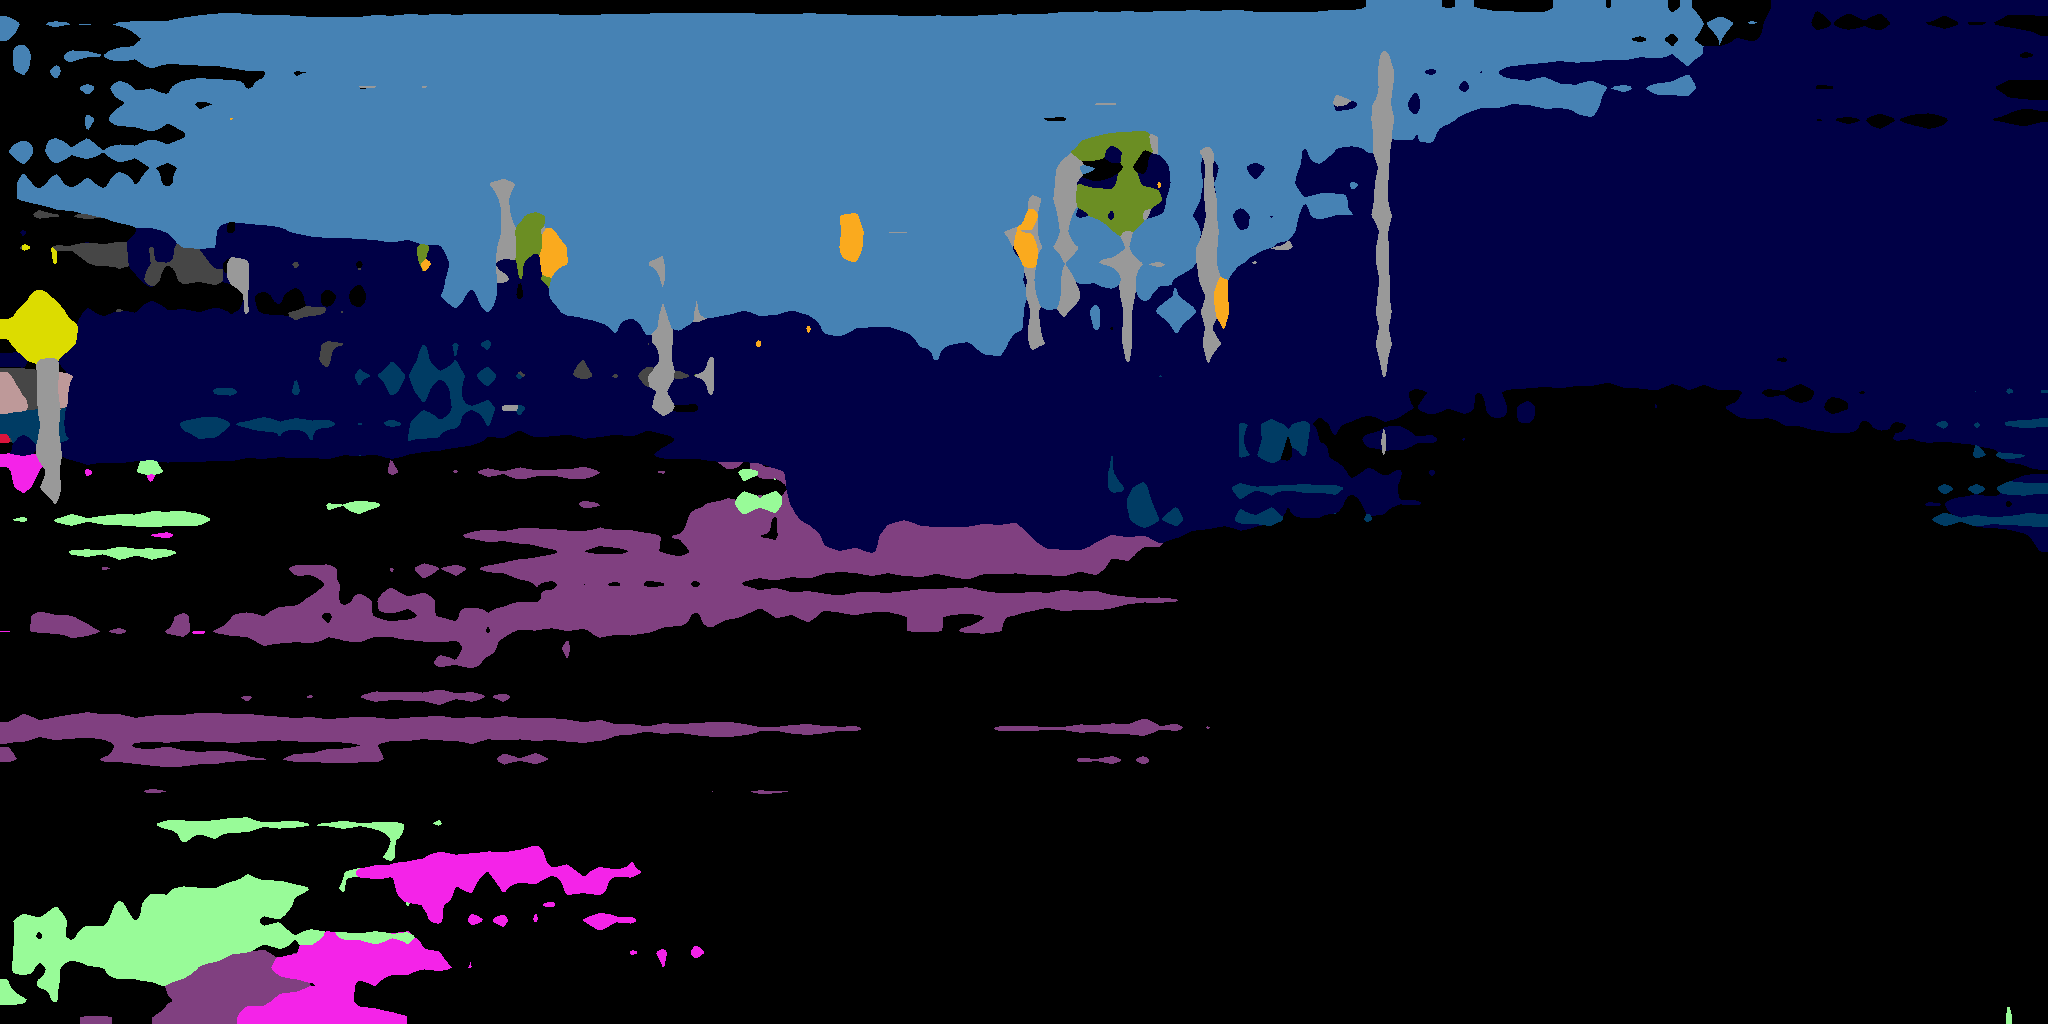
\includegraphics[width=\textwidth]{images/evaluation/SG-GAN_pred_labels_train.png}
		\end{minipage} \\
		%\multicolumn{2}{c}{} \\
		\multicolumn{1}{c}{} & (translated) Image & (predicted) Label map
	\end{tabular} 
	\caption{An example of an image containing a train. Comparing the images translated by the different methods and the corresponding semantic segmentation. It is easy to see that CyCADA performs best in this comparison on semantic segmentation of the train (colored dark teal).}
	\label{table:train}
\end{table}

\begin{table}
	\centering
	\begin{tabular}{|c|c|c|c|c|}
		\multicolumn{5}{c}{\textbf{category scores}}\\
		\hline
		\multicolumn{1}{c}{} & \multicolumn{4}{c}{Methods}\\
		\cline{2-5}
		\multicolumn{1}{c|}{category} & GTA5 & CycleGAN & CyCADA & SG-GAN\\ 
		\hline
		construction & 0.636 & 0.598 & \textbf{0.674} & 0.628\\ 
		\hline 
		flat & 0.740 & 0.861 & \textbf{0.894} & 0.735\\ 
		\hline 
		human & \textbf{0.546} & 0.402 & 0.440 & 0.487\\ 
		\hline 
		nature & 0.543 & 0.615 & \textbf{0.622} & 0.585\\ 
		\hline 
		object & \textbf{0.085} & 0.067 & 0.073 & 0.080\\ 
		\hline 
		sky & \textbf{0.872} & 0.822 & 0.832 & 0.644\\ 
		\hline 
		vehicle & 0.641 & 0.557 & \textbf{0.680} & 0.609\\ 
		\hline \hline
		average & 0.580 & 0.560 & \textbf{0.602} & 0.538\\
		\hline
		\multicolumn{5}{c}{}\\
		\multicolumn{5}{c}{\textbf{class scores}}\\
		\hline
		\multicolumn{1}{c}{} & \multicolumn{4}{c}{Methods}\\
		\cline{2-5}
		\multicolumn{1}{c|}{class} & GTA5 & CycleGAN & CyCADA & SG-GAN\\ 
		\hline
		bicycle & \textbf{0.100} & 0.038 & 0.041 & 0.051\\ 
		\hline 
		building & 0.620 & 0.509 & \textbf{0.634} & 0.513\\ 
		\hline 
		bus & 0.209 & 0.136 & 0.190 & \textbf{0.257}\\ 
		\hline 
		car & 0.627 & 0.570 & 0.640 & \textbf{0.642}\\ 
		\hline 
		fence & 0.100 & 0.102 & \textbf{0.125} & 0.083\\ 
		\hline 
		motorcycle & 0.195 & 0.125 & \textbf{0.297} & 0.256\\ 
		\hline 
		person & \textbf{0.524} & 0.369 & 0.398 & 0.461\\ 
		\hline 
		pole & 0.0 & 0.0 & 0.0 & 0.0\\ 
		\hline 
		rider & \textbf{0.312} & 0.160 & 0.144 & 0.247\\ 
		\hline 
		road & 0.658 & 0.752 & \textbf{0.775} & 0.631\\ 
		\hline 
		sidewalk & \textbf{0.434} & 0.365 & 0.339 & 0.381\\ 
		\hline 
		sky & \textbf{0.872} & 0.822 & 0.832 & 0.644\\ 
		\hline 
		terrain & 0.282 & 0.361 & \textbf{0.374} & 0.292\\ 
		\hline 
		traffic light & \textbf{0.210} & 0.178 & 0.187 & 0.185\\ 
		\hline 
		traffic sign & 0.090 & 0.126 & 0.120 & \textbf{0.158}\\ 
		\hline 
		train & 0.025 & 0.115 & \textbf{0.280} & 0.222\\ 
		\hline 
		truck & 0.387 & 0.371 & \textbf{0.511} & 0.332\\ 
		\hline 
		vegetation & 0.595 & 0.620 & 0.595 & \textbf{0.653}\\ 
		\hline 
		wall & 0.162 & 0.186 & \textbf{0.225} & 0.186\\ 
		\hline \hline 
		average & 0.337 & 0.311 & \textbf{0.353} & 0.326\\
		\hline
	\end{tabular} 
	\caption{Intersection over Union results for evaluation on untranslated GTA5 images and translated images by CycleGAN, CyCADA and SG-GAN respectively. Rounded to 3 decimal places. Maximum value per row is illustrated in big font.}
	\label{table:results_quant}
\end{table}

\subsection{Qualitative}
Table \ref{table:results_qual} shows a qualitative comparison for a single frame translated through each method and with corresponding predicted label map. One can see that all of the techniques darkened the overall appearance of the image while SG-GAN still has brighter color than CycleGAN and CyCADA. CyCADA smooths out the road the most out of all of the techniques and SG-GAN least. SG-GAN has a lot of noisy structure in the translated images. Also they have a bright glow between the sky and other semantic classes. The only technique that learned the Mercedes star and generates it in most of the images is CyCADA. Overall, the SG-GAN images look very sharp and close to the original GTA5 images while CycleGAN and CyCADA smooth out the textures more. The pedestrians on the right side of the images are more clearly generated in CyCADA than CycleGAN. The predicted label map of the ground truth GTA5 image clearly shows that the DeepLabv3 model trained on Cityscapes performs worse in the synthetic domain. For SG-GAN it predicts large portions of the road as sidewalks and generates noisy label images. The DeepLabv3 model is able to successfully predict streets and sidewalks for CyCADA and CycleGAN images. While it predicts some regions other than the ego car as void for SG-GAN and CycleGAN, CyCADA only has one small region that it cannot predict as belonging to one of the main classes. The CyCADA label map contains more vegetation than the ground truth. 

% void
\definecolor{black}{rgb}{0, 0, 0} % unlabeled, ego vehicle, rectification border, out of roi, static

%flat
\definecolor{purple}{rgb}{0.5, 0.25, 0.5} %road
\definecolor{lightpurple}{rgb}{0.96, 0.14, 0.91} %sidewalk

% construction
\definecolor{grey}{rgb}{0.27, 0.27, 0.27} % building
\definecolor{bluepurple}{rgb}{0.4, 0.4, 0.61} % wall
\definecolor{darkerskin}{rgb}{0.75, 0.6, 0.6} % fence

%object
\definecolor{grey2}{rgb}{0.6, 0.6, 0.6} % pole
\definecolor{orange}{rgb}{0.98, 0.67, 0.12} % traffic light
\definecolor{lightgreen}{rgb}{0.86, 0.86, 0} % traffic sign

%nature
\definecolor{green}{rgb}{0.42, 0.56, 0.14} % vegetation
\definecolor{brightgreen}{rgb}{0.60, 0.98, 0.60} % terrain

%sky
\definecolor{blue}{rgb}{0.27, 0.51, 0.71} % sky

%human
\definecolor{red}{rgb}{0.86, 0.08, 0.24} % person
\definecolor{fullred}{rgb}{1, 0, 0} % rider

%vehicle
\definecolor{darkblue}{rgb}{0, 0, 0.56} % car
\definecolor{blueblack}{rgb}{0, 0, 0.27} % truck
\definecolor{paleblue}{rgb}{0, 0.24, 0.39} % bus
\definecolor{palegreenblue}{rgb}{0, 0.31, 0.39} % train
\definecolor{brightblue}{rgb}{0, 0, 0.90} % motorcycle
\definecolor{brownred}{rgb}{0.47, 0.04, 0.13} % bicycle

\begin{table}
	\centering
	\setlength\tabcolsep{1.5pt}
%	\begin{tabular}{cc||c}
%		\rotatebox[origin=c]{90}{\thead{GTA \\ (Ground Truth)}} & 
%		\begin{minipage}[c]{0.45\textwidth}
%			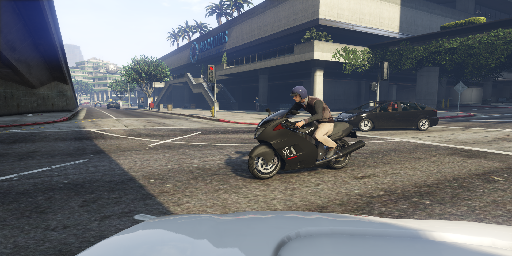
\includegraphics[width=\textwidth]{images/evaluation/00991_leftImg8bit.png}
%		\end{minipage} & 
%		\begin{minipage}[c]{0.45\textwidth}
%			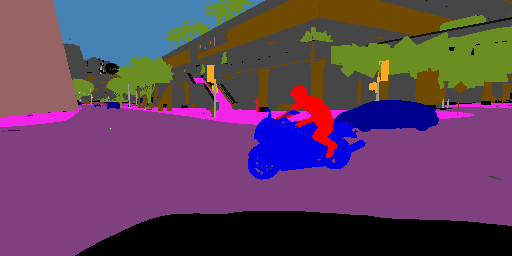
\includegraphics[width=\textwidth]{images/evaluation/00991_gtFine_labelIds.png}
%		\end{minipage}\\
%		\hline
%		\hline
%		\rotatebox[origin=c]{90}{GTA} &
%		\multicolumn{1}{c||}{} &
%		\begin{minipage}[c]{0.45\textwidth}
%			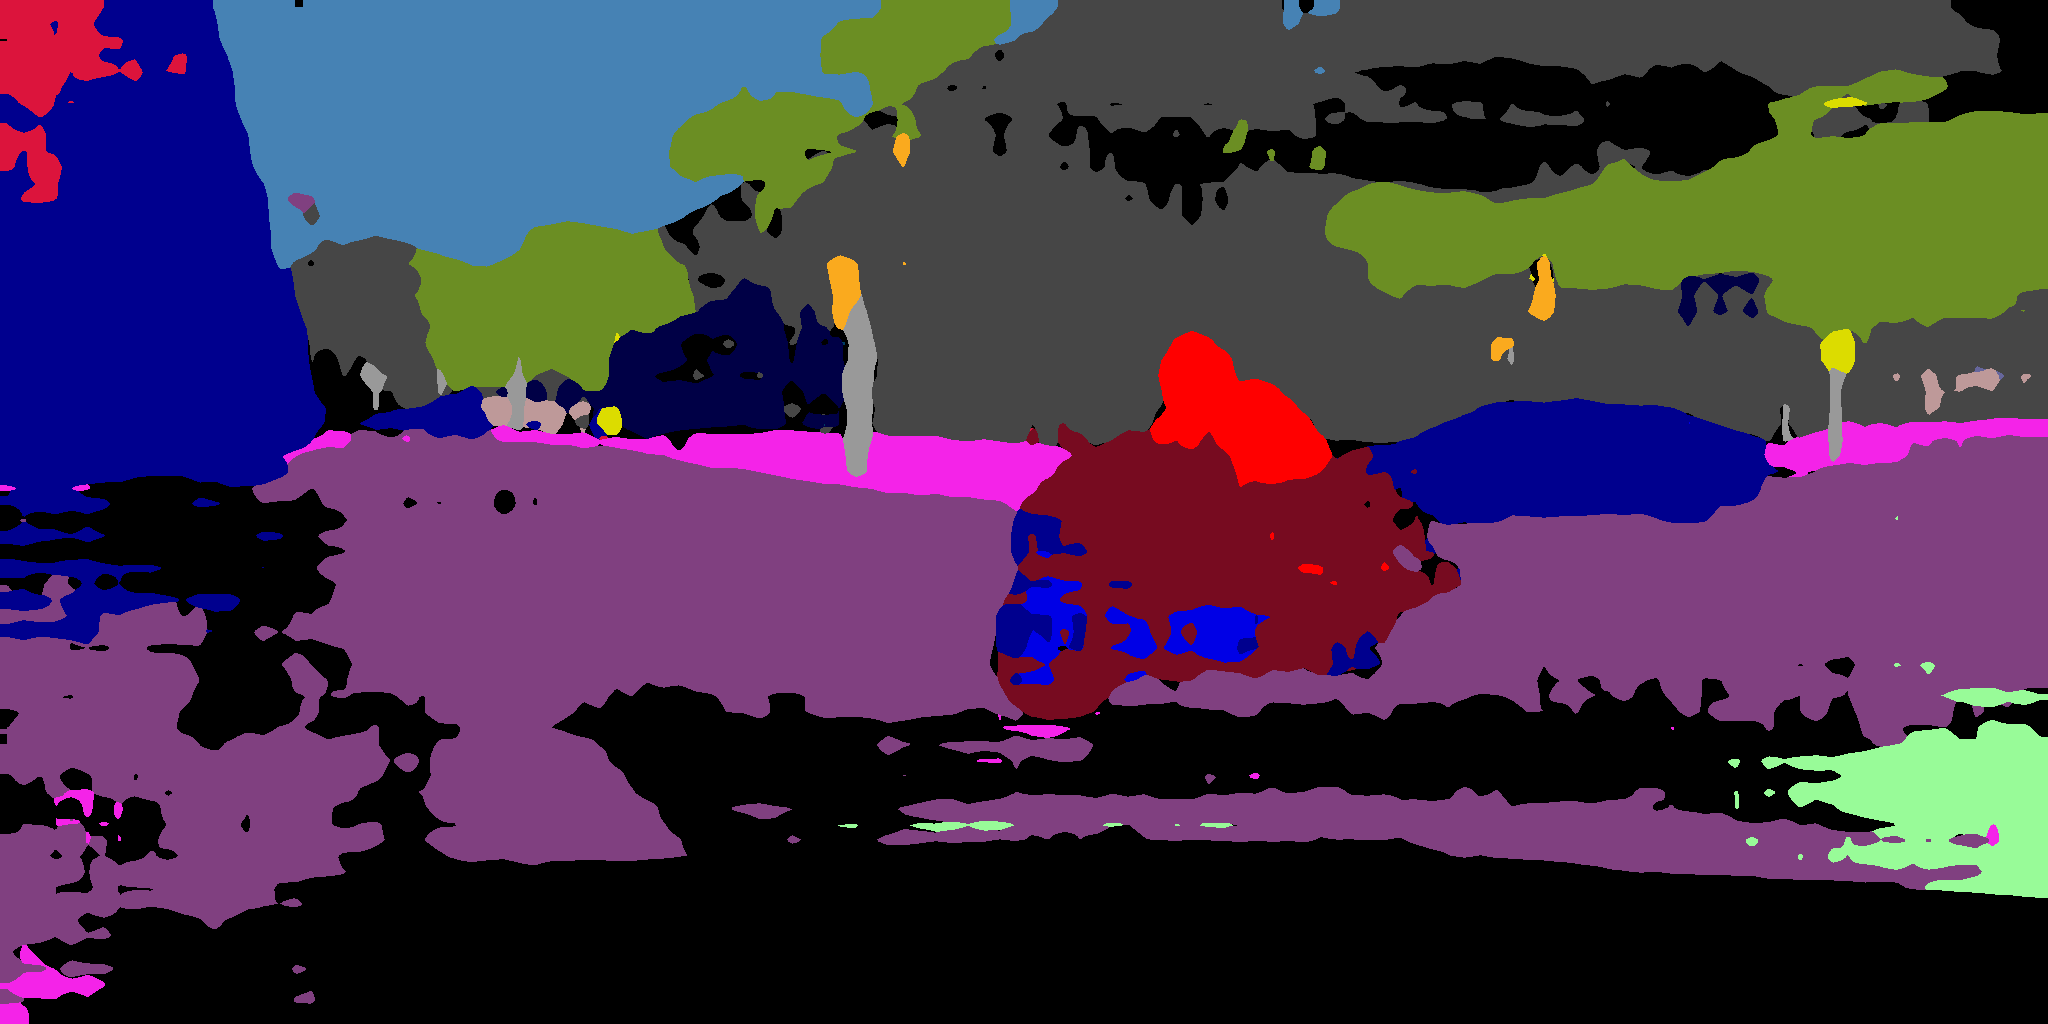
\includegraphics[width=\textwidth]{images/evaluation/gta_00991_pred_label_img.png}
%		\end{minipage}\\
%		\rotatebox[origin=c]{90}{CycleGAN} &
%		\begin{minipage}[c]{0.45\textwidth}
%			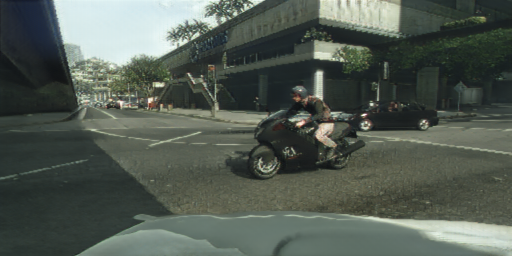
\includegraphics[width=\textwidth]{images/evaluation/CycleGAN_00991_leftImg8bit.png}
%		\end{minipage} &
%		\begin{minipage}[c]{0.45\textwidth}
%			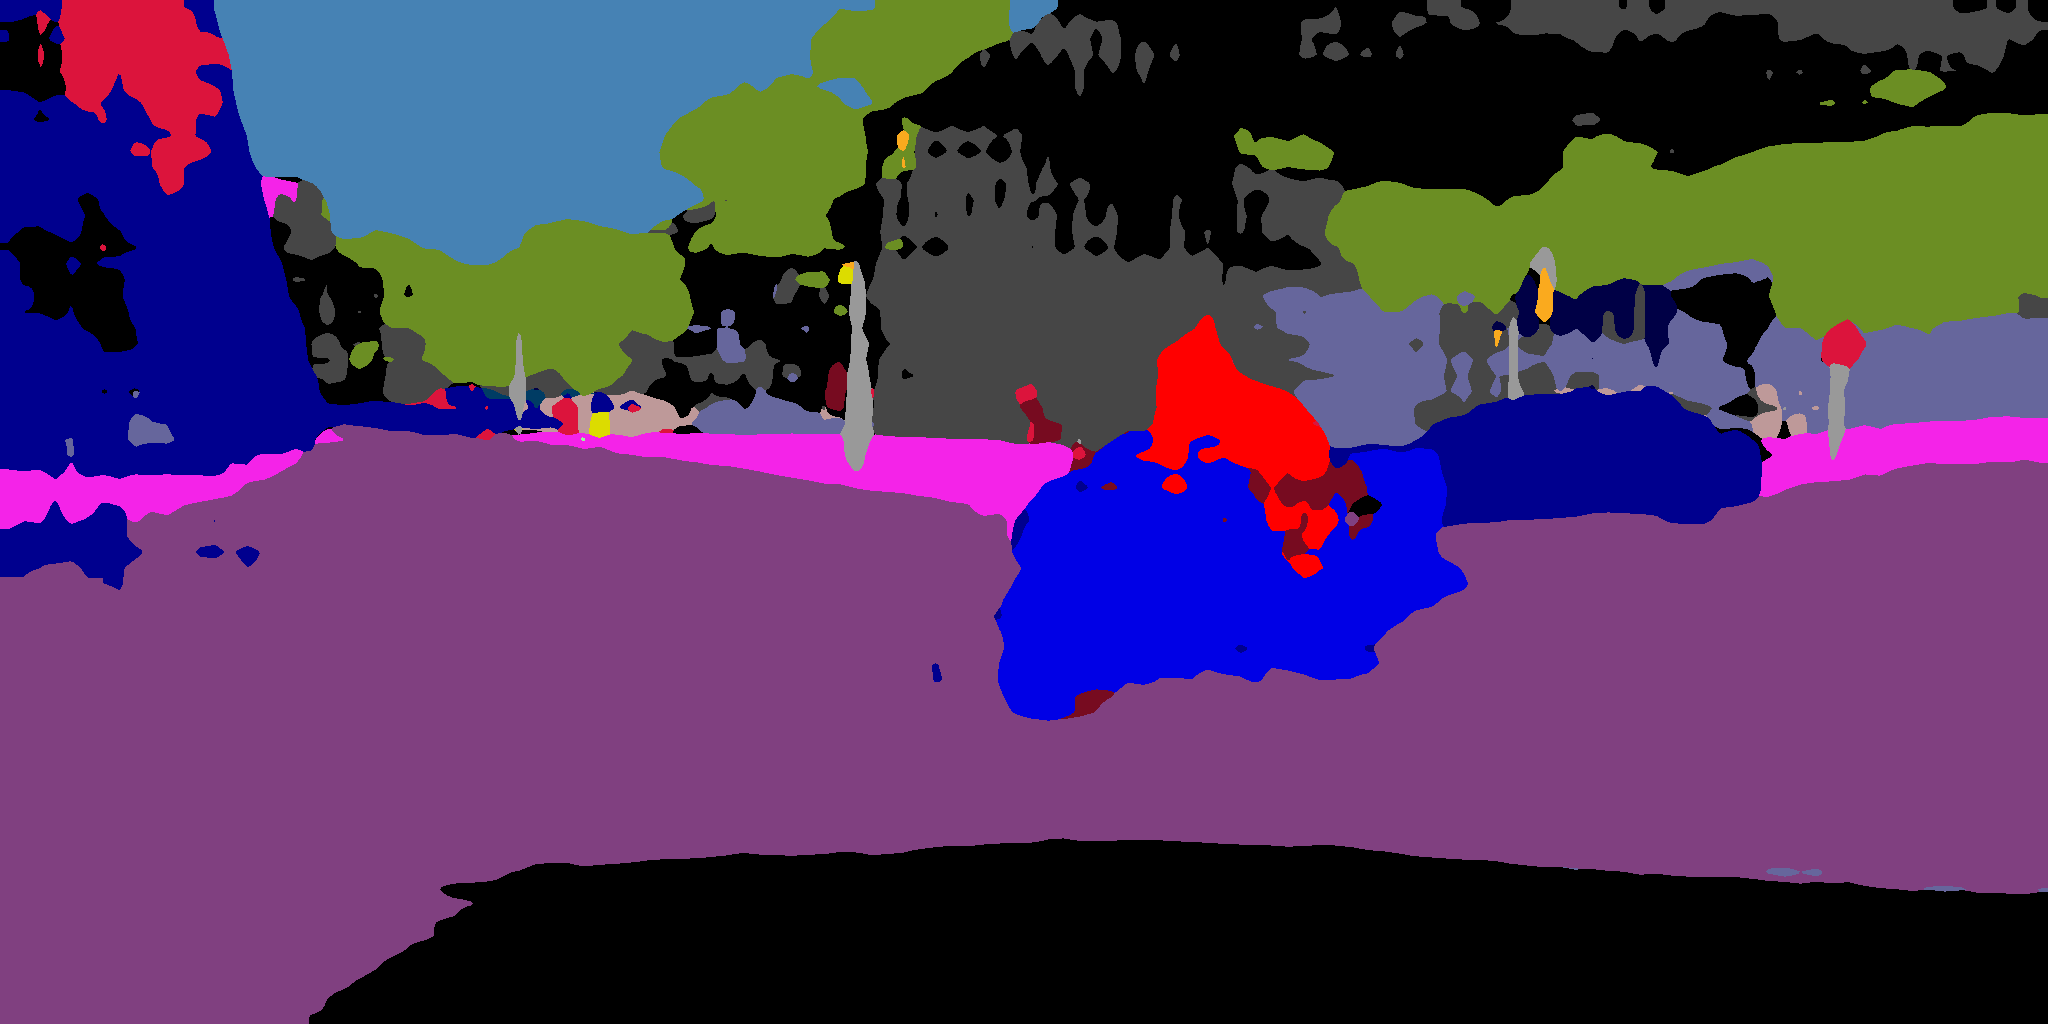
\includegraphics[width=\textwidth]{images/evaluation/CycleGAN_00991_pred_label_img.png}
%		\end{minipage}\\
%		\rotatebox[origin=c]{90}{CyCADA} &
%		\begin{minipage}[c]{0.45\textwidth} 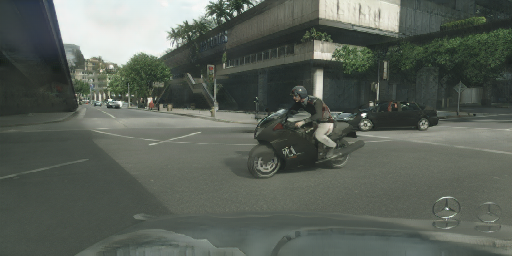
\includegraphics[width=\textwidth]{images/evaluation/CyCADA_00991_leftImg8bit.png} 
%		\end{minipage}& 
%		\begin{minipage}[c]{0.45\textwidth}
%			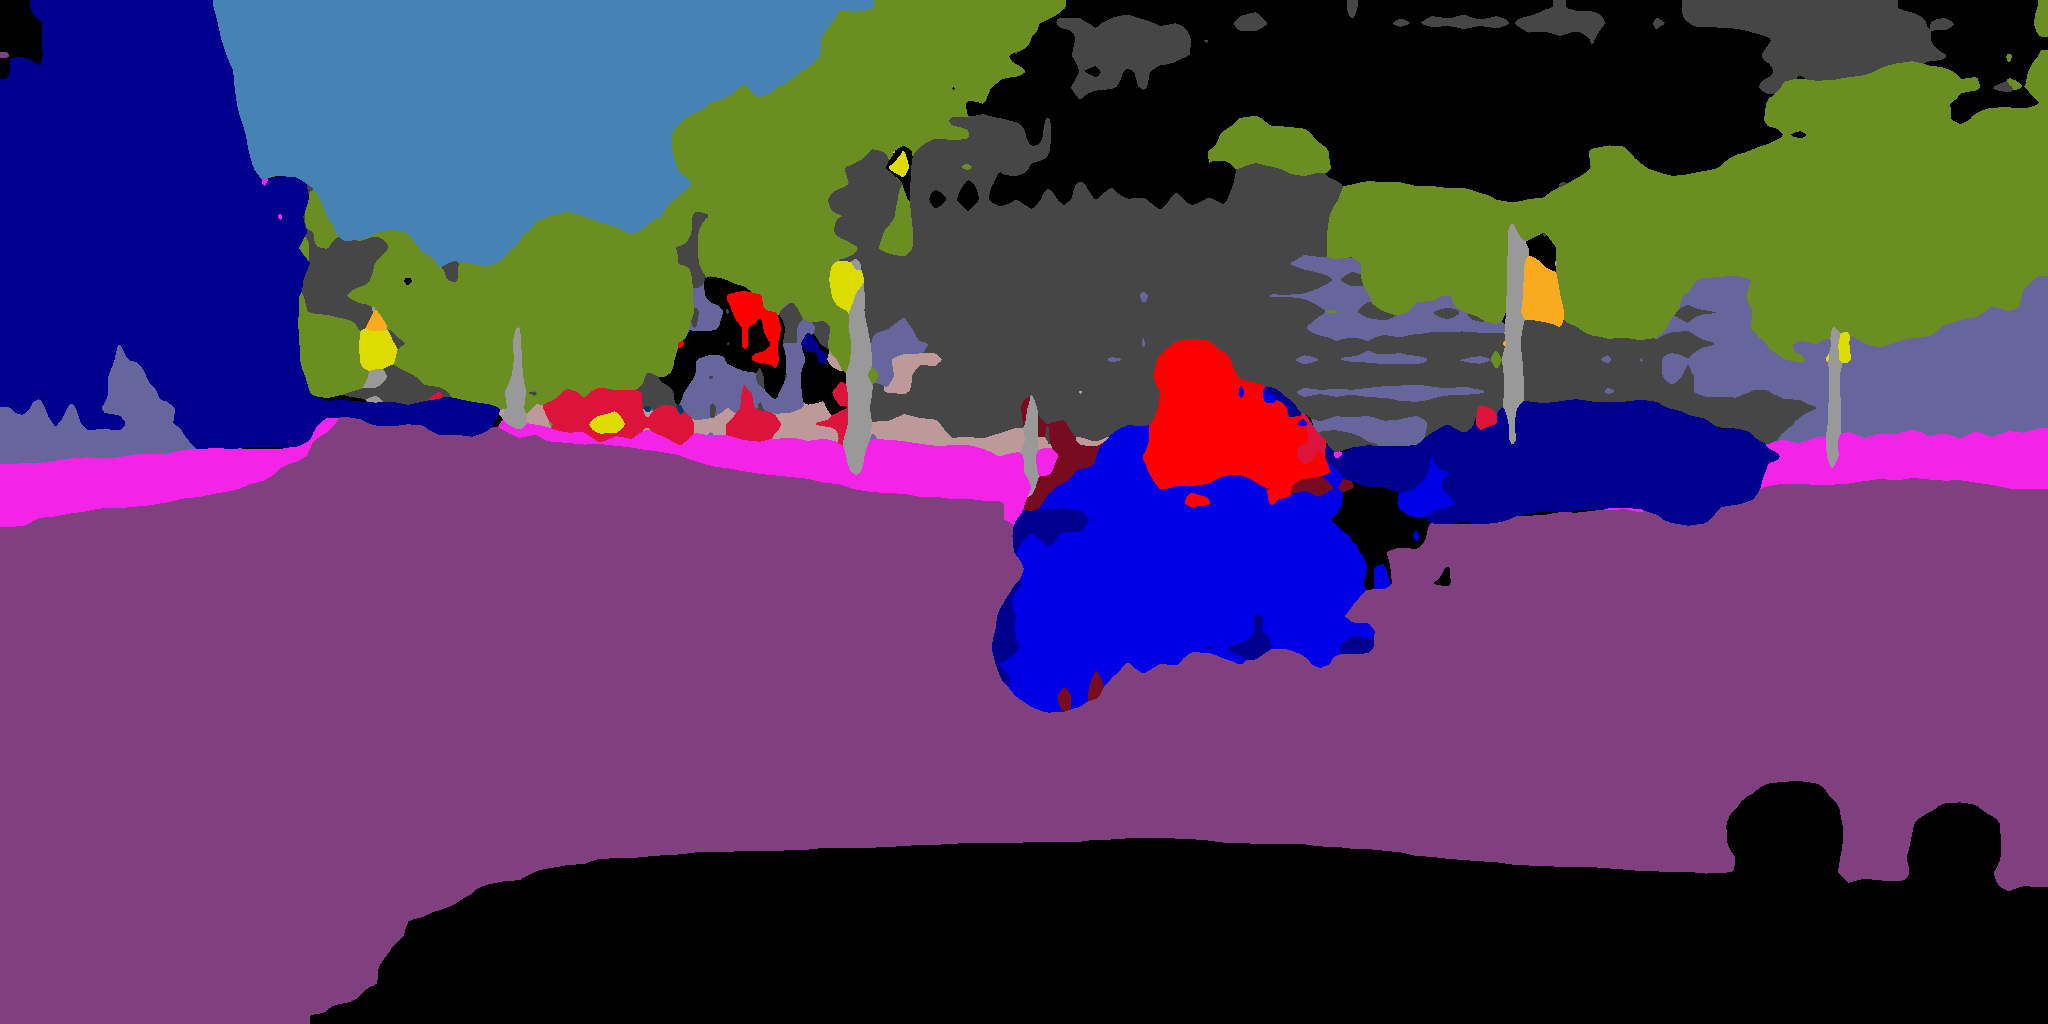
\includegraphics[width=\textwidth]{images/evaluation/CyCADA_00991_pred_label_img.png}
%		\end{minipage}\\
%		\rotatebox[origin=c]{90}{SG-GAN} &
%		\begin{minipage}[c]{0.45\textwidth} 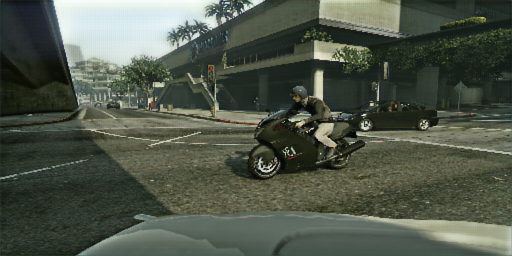
\includegraphics[width=\textwidth]{images/evaluation/SG-GAN_00991_leftImg8bit.png}
%		\end{minipage} & 
%		\begin{minipage}[c]{0.45\textwidth}
%			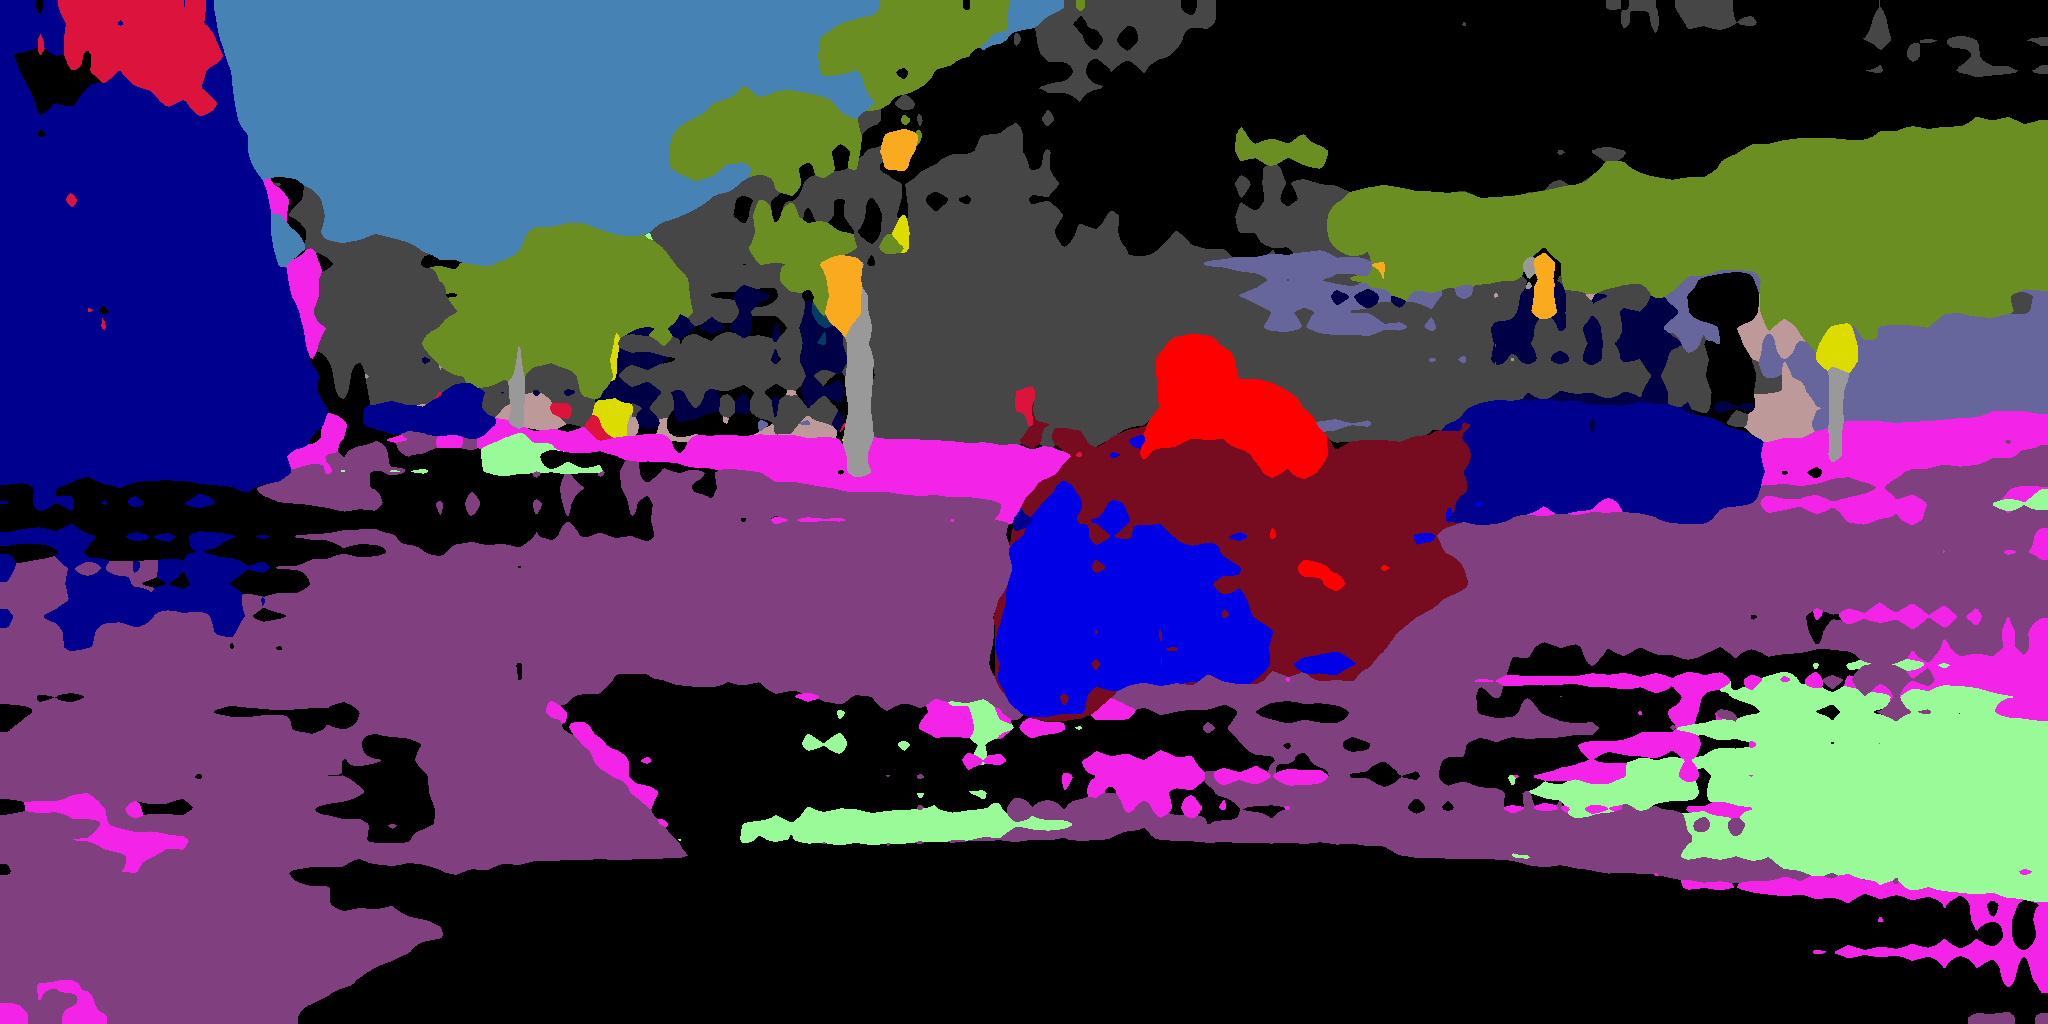
\includegraphics[width=\textwidth]{images/evaluation/SG-GAN_00991_pred_label_img.png}
%		\end{minipage} \\
%		%\multicolumn{2}{c}{} \\
%		\multicolumn{1}{c}{} & (translated) Image & (predicted) Label map
%	\end{tabular}
		\begin{tabular}{cc||c}
		\rotatebox[origin=c]{90}{\thead{GTA5 \\ (Ground Truth)}} & 
		\begin{minipage}[c]{0.45\textwidth}
			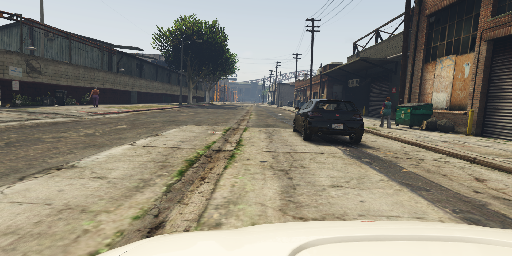
\includegraphics[width=\textwidth]{images/evaluation/GTA_gt_image.png}
		\end{minipage} & 
		\begin{minipage}[c]{0.45\textwidth}
			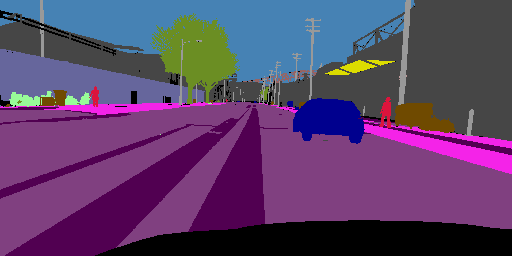
\includegraphics[width=\textwidth]{images/evaluation/GTA_gt_label.png}
		\end{minipage}\\
		\hline
		\hline
		\rotatebox[origin=c]{90}{GTA5} &
		\multicolumn{1}{c||}{} &
		\begin{minipage}[c]{0.45\textwidth}
			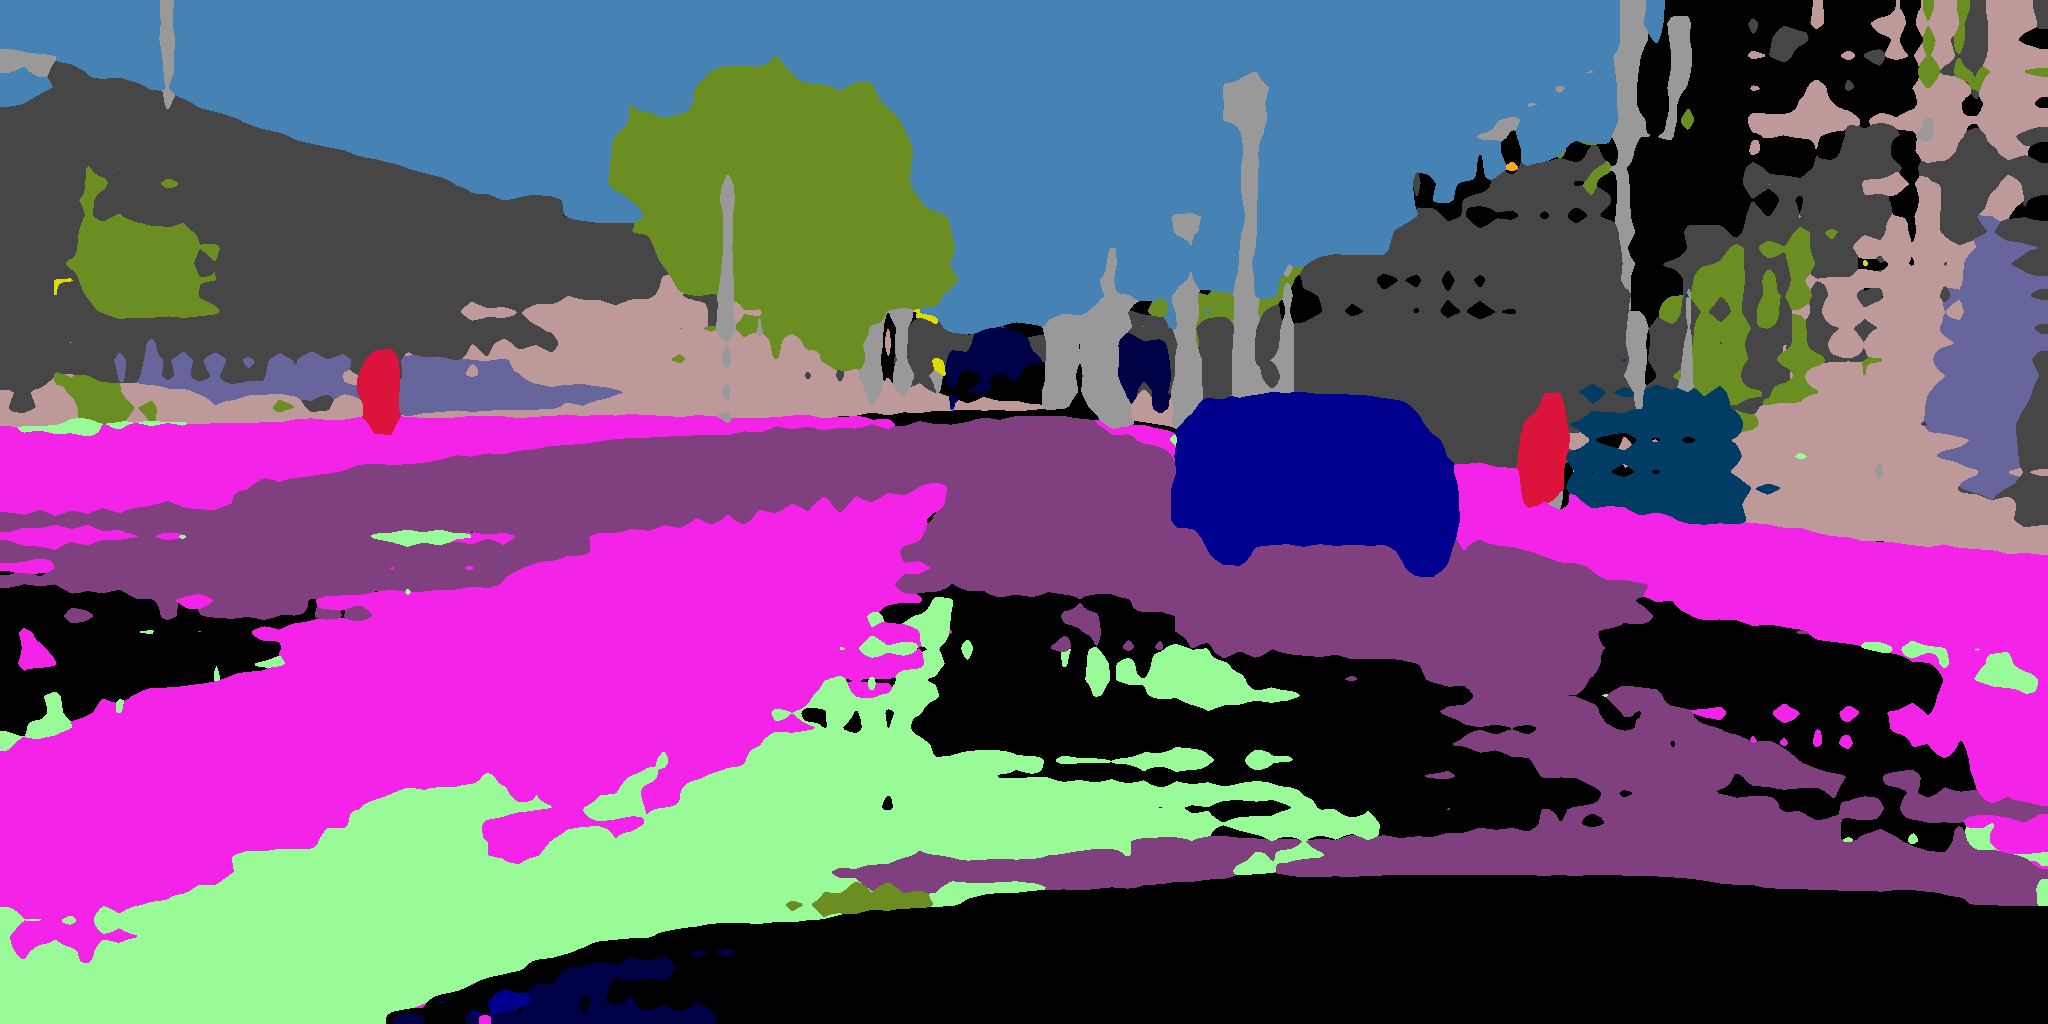
\includegraphics[width=\textwidth]{images/evaluation/GTA_pred_labels.png}
		\end{minipage}\\
		\rotatebox[origin=c]{90}{CycleGAN} &
		\begin{minipage}[c]{0.45\textwidth}
			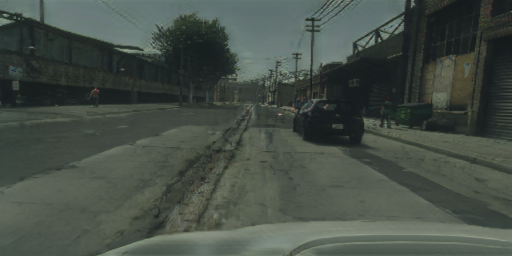
\includegraphics[width=\textwidth]{images/evaluation/CycleGAN_translated.png}
		\end{minipage} &
		\begin{minipage}[c]{0.45\textwidth}
			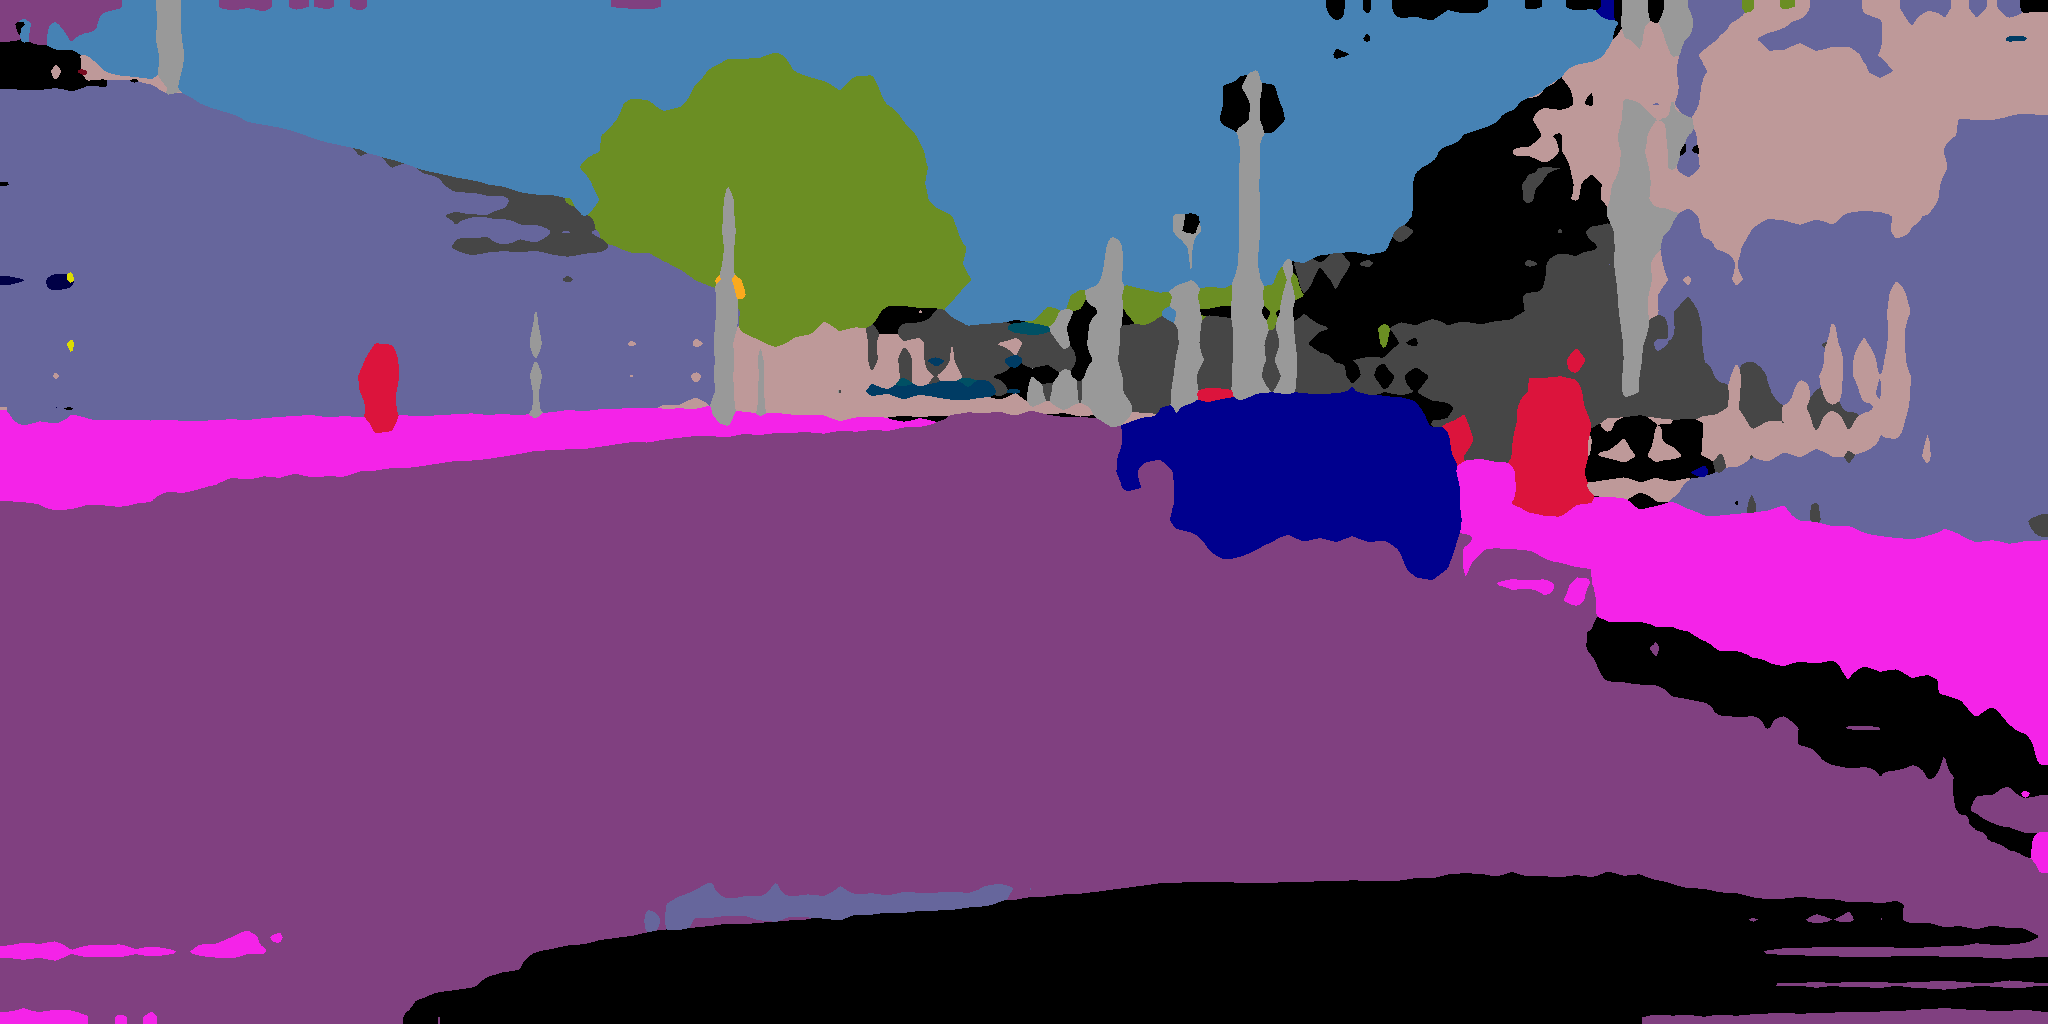
\includegraphics[width=\textwidth]{images/evaluation/CycleGAN_pred_labels.png}
		\end{minipage}\\
		\rotatebox[origin=c]{90}{CyCADA} &
		\begin{minipage}[c]{0.45\textwidth} 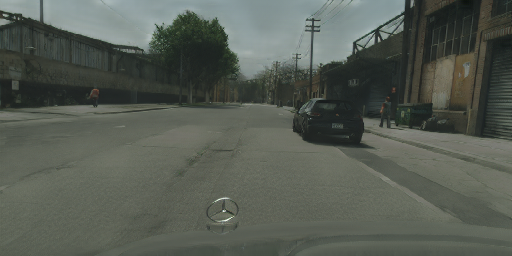
\includegraphics[width=\textwidth]{images/evaluation/CyCADA_translated.png} 
		\end{minipage}& 
		\begin{minipage}[c]{0.45\textwidth}
			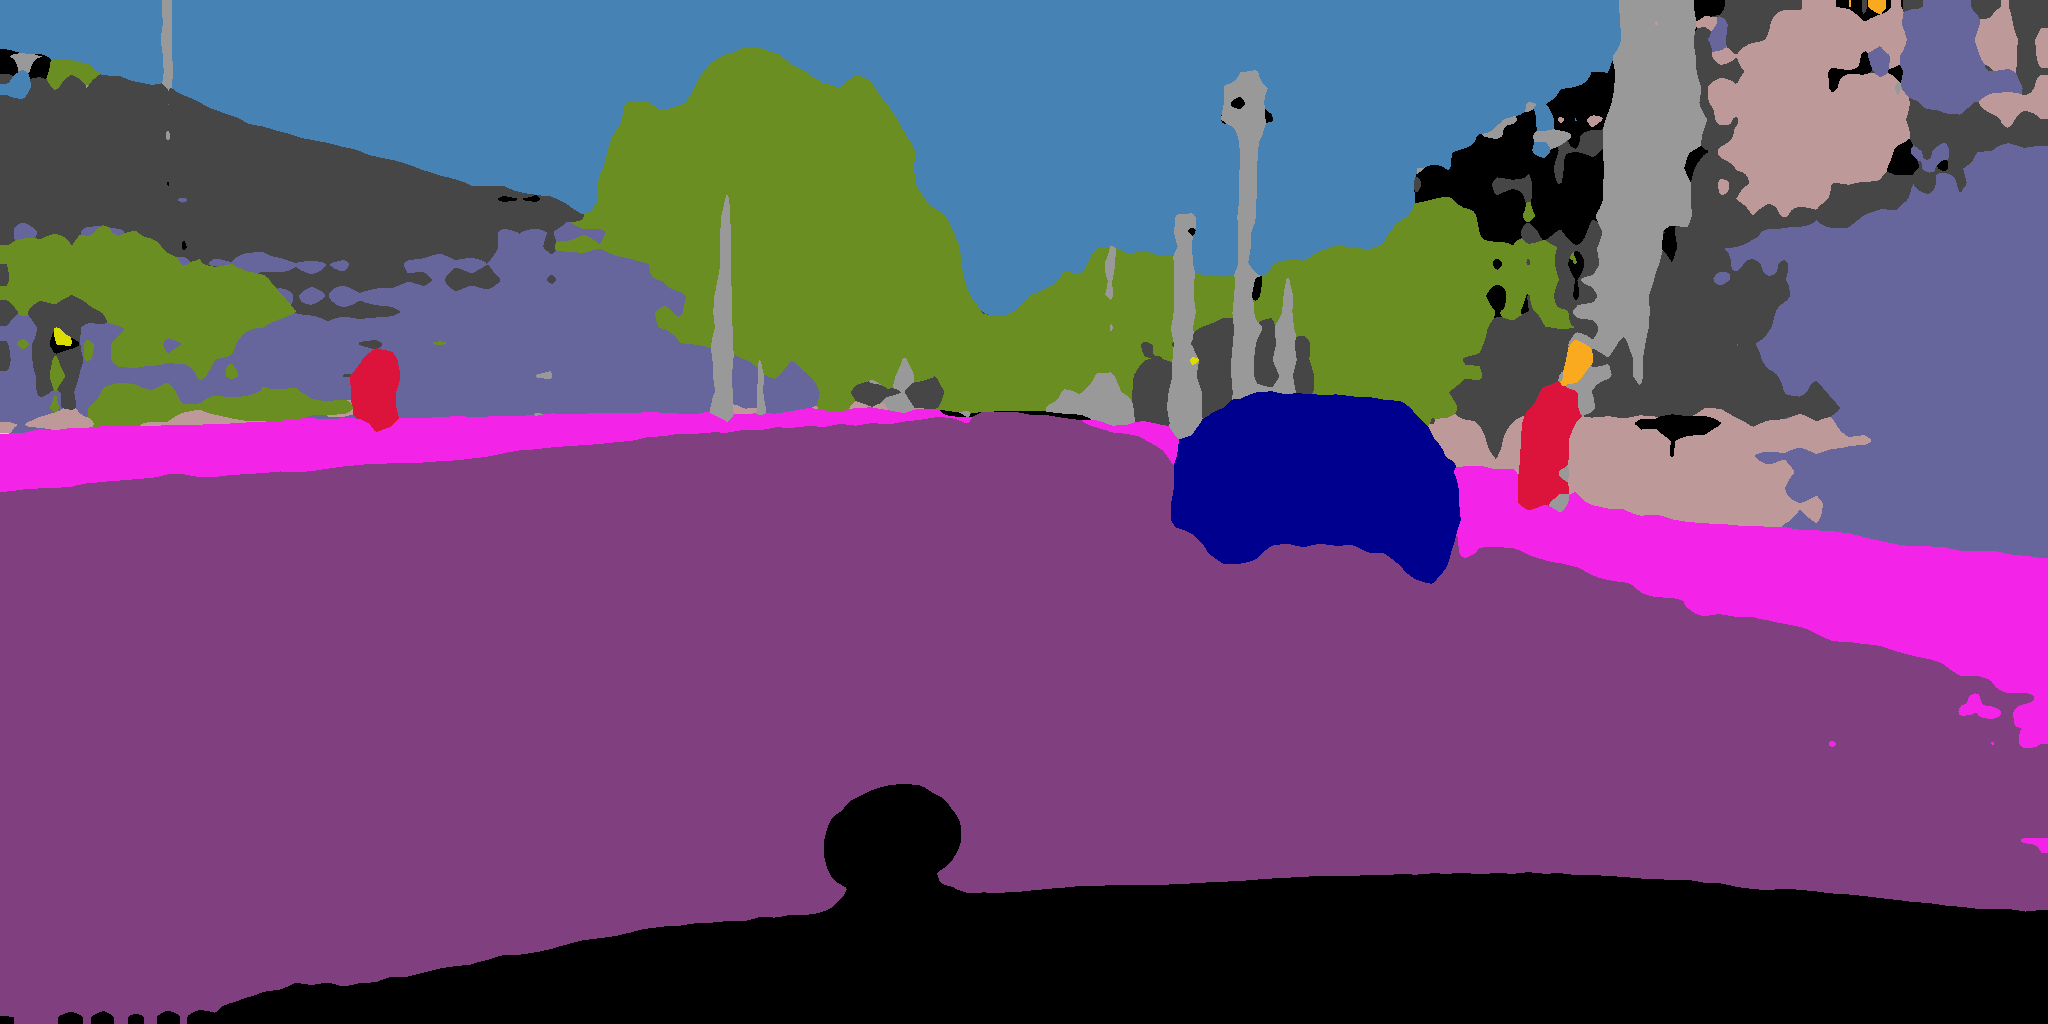
\includegraphics[width=\textwidth]{images/evaluation/CyCADA_pred_labels.png}
		\end{minipage}\\
		\rotatebox[origin=c]{90}{SG-GAN} &
		\begin{minipage}[c]{0.45\textwidth} 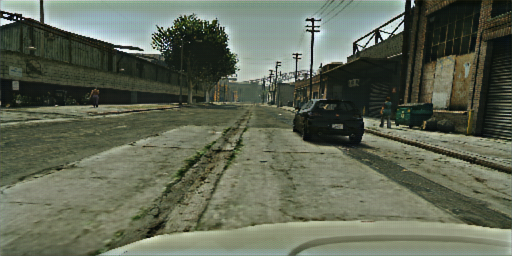
\includegraphics[width=\textwidth]{images/evaluation/SG-GAN_translated.png}
		\end{minipage} & 
		\begin{minipage}[c]{0.45\textwidth}
			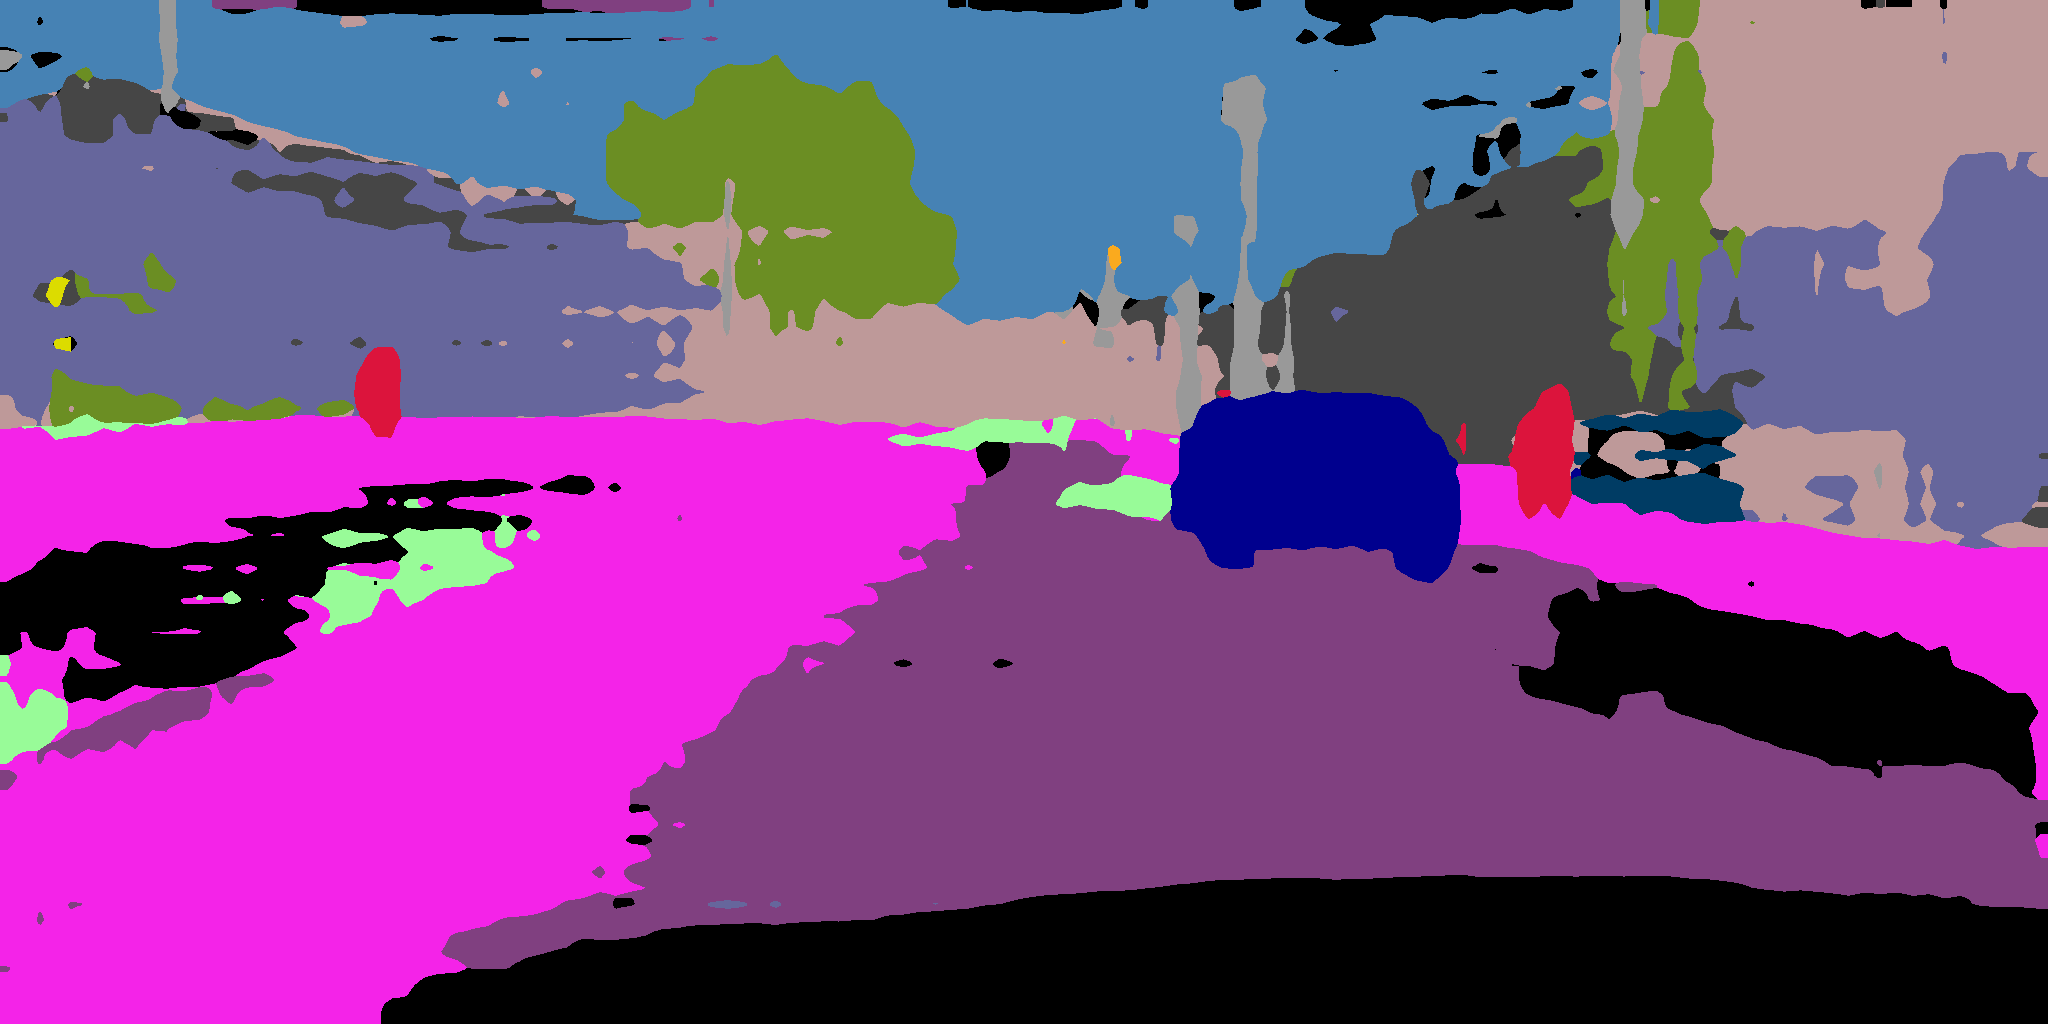
\includegraphics[width=\textwidth]{images/evaluation/SG-GAN_pred_labels.png}
		\end{minipage} \\
		%\multicolumn{2}{c}{} \\
		\multicolumn{1}{c}{} & (translated) Image & (predicted) Label map
	\end{tabular} 
	\caption{Ground Truth image and corresponding Ground Truth label map from the GTA5 dataset (top) and the images translated by the different techniques (left side) with their corresponding predicted label maps (right side)}
	\label{table:results_qual}
	\bigskip
	\centering
	\begin{tabular}{cccccccccccccccccccc}
		\raisebox{-.25\height}{\textcolor{black}{\rule{0.5cm}{0.5cm}}} &
		\raisebox{-.25\height}{\textcolor{purple}{\rule{0.5cm}{0.5cm}}} &
		\raisebox{-.25\height}{\textcolor{lightpurple}{\rule{0.5cm}{0.5cm}}} &
		\raisebox{-.25\height}{\textcolor{grey}{\rule{0.5cm}{0.5cm}}} &
		\raisebox{-.25\height}{\textcolor{bluepurple}{\rule{0.5cm}{0.5cm}}} &
		\raisebox{-.25\height}{\textcolor{darkerskin}{\rule{0.5cm}{0.5cm}}} &
		\raisebox{-.25\height}{\textcolor{grey2}{\rule{0.5cm}{0.5cm}}} &
		\raisebox{-.25\height}{\textcolor{orange}{\rule{0.5cm}{0.5cm}}} &
		\raisebox{-.25\height}{\textcolor{lightgreen}{\rule{0.5cm}{0.5cm}}} &
		\raisebox{-.25\height}{\textcolor{green}{\rule{0.5cm}{0.5cm}}} &
		\raisebox{-.25\height}{\textcolor{brightgreen}{\rule{0.5cm}{0.5cm}}} &
		\raisebox{-.25\height}{\textcolor{blue}{\rule{0.5cm}{0.5cm}}} &
		\raisebox{-.25\height}{\textcolor{red}{\rule{0.5cm}{0.5cm}}} &
		\raisebox{-.25\height}{\textcolor{fullred}{\rule{0.5cm}{0.5cm}}} &
		\raisebox{-.25\height}{\textcolor{darkblue}{\rule{0.5cm}{0.5cm}}} &
		\raisebox{-.25\height}{\textcolor{blueblack}{\rule{0.5cm}{0.5cm}}} &
		\raisebox{-.25\height}{\textcolor{paleblue}{\rule{0.5cm}{0.5cm}}} &
		\raisebox{-.25\height}{\textcolor{palegreenblue}{\rule{0.5cm}{0.5cm}}} &
		\raisebox{-.25\height}{\textcolor{brightblue}{\rule{0.5cm}{0.5cm}}} &
		\raisebox{-.25\height}{\textcolor{brownred}{\rule{0.5cm}{0.5cm}}} \\
		\rotatebox[origin=r]{90}{void} & \rotatebox[origin=r]{90}{road} & \rotatebox[origin=r]{90}{sidewalk} & \rotatebox[origin=r]{90}{building} & \rotatebox[origin=r]{90}{wall} & \rotatebox[origin=r]{90}{fence} & \rotatebox[origin=r]{90}{pole} & \rotatebox[origin=r]{90}{traffic light} & \rotatebox[origin=r]{90}{traffic sign} & \rotatebox[origin=r]{90}{vegetation} & \rotatebox[origin=r]{90}{terrain} & \rotatebox[origin=r]{90}{sky} & \rotatebox[origin=r]{90}{person} & \rotatebox[origin=r]{90}{rider} & \rotatebox[origin=r]{90}{car} & \rotatebox[origin=r]{90}{truck} & \rotatebox[origin=r]{90}{bus} & \rotatebox[origin=r]{90}{train} & \rotatebox[origin=r]{90}{motorcycle} & \rotatebox[origin=r]{90}{bicycle}
	\end{tabular} 
	\caption{Color coding of semantic classes used in semantic segmentation label maps.}
	\label{table:semseg_colors}
	\setlength\tabcolsep{6pt}
\end{table}


\newpage

\section{Discussion}
CyCADA performed best on average for both category and class scores in this comparison. From the translated images used in this comparison it looks like CyCADA was able to smoothen textures more than the other methods giving them a more realistic look. This is especially obvious when looking at the ``flat'' category scores where it improves semantic segmentation by as much as $15.4\%$. The untranslated GTA5 images having the best scores for human, sky and object categories is probably due to noise and artifacts generated by the adaptation techniques. This results in reduced details for instances of the human category which is generally already smaller (pixel-wise) than the other categories. SG-GAN creates a lot of noise into the sky which makes correct prediction of sky labels a lot harder for the DeepLabv3 model. SG-GAN performing best for cars and buses might be due to generating distinct pixels around semantic boundaries which may result in better distinction between instances of cars and buses far in the background and their surroundings. The ``glow'' is especially visible between the sky and its neighboring semantic classes. This might be the reason for SG-GAN to perform best for traffic signs as they are easier to seperate from the background. Overall, the results are not as expected. All of the techniques compared in this work show in their corresponding papers that they improve the performance of semantic segmentation models compared to unadapted images for GTA5 to Cityscapes domain adaptation. This is not the case here. This is probably due to the models used in this work not being the ones the authors actually used in their works. Therefore, it can't be ensured that they were trained the way the authors describe which may result in the decrease in average performance for CycleGAN and SG-GAN. 

\chapter{Conclusion}
\label{sec:conclusion}


\section{Outlook and Future Work}


\appendix
\chapter{Blub}

\bibliographystyle{alpha}
\bibliography{bibliography}

\end{document}

